\documentclass[11pt]{article}
\usepackage{graphicx}
\graphicspath{{/Users/justindoty/Documents/Research/Dissertation/Production_QR_Proxy/Code/}}
\usepackage{graphics}
\usepackage{amsfonts}
\usepackage{amsmath}
\usepackage{amstext}
\usepackage{tabularx}
\usepackage{mathrsfs}
\usepackage{subfigure}
\usepackage{color}
\usepackage{lscape}
\usepackage{longtable}
\usepackage{bm}
\usepackage{bbm}
\usepackage{chngcntr}
\usepackage{setspace}
\usepackage{caption}
\usepackage{float}
\usepackage{multirow}
\usepackage{booktabs}
\usepackage{natbib}
\usepackage{fancyvrb}
\usepackage{enumitem}
\usepackage[multiple]{footmisc}
\newtheorem{assump}{Assumption}[section]
\newtheorem{lemma}{Lemma}[section]
\newtheorem{theorem}{Theorem}[section]


\usepackage[multiple]{footmisc}

%Set margins and text size
\setlength{\textwidth}{6.5in} \setlength{\textheight}{8.8in}
\setlength{\topmargin}{-0.5in}
\setlength{\oddsidemargin}{-0.01in}{}
\setlength{\parskip}{1.6mm}
\parskip=.06in
{}
%Some useful short-cuts
\def\argmax{\mathop{\rm arg\,max}}
\def\argmin{\mathop{\rm arg\,min}}



\setcounter{section}{0} % starts numbering section 1start_value=[0.498,-0.2874,0.4314,0.5444];

\setcounter{page}{1}



% \usepackage[pdftex]{hyperref}
\begin{document}

\title{Heterogeneity in Firms: \\
A Proxy Variable Approach for Quantile Production Functions
%\footnote{}
}

\author{Justin Doty\thanks{Department of Economics, University of Iowa, S321 Pappajohn Business Building, 21 E Market St, Iowa City, IA 52242. Email: \texttt{justin-doty@uiowa.edu}} and Suyong Song\thanks{Department of Economics and Finance, University of Iowa, W360 Pappajohn Business Building, 21 E Market St, Iowa City, IA 52242. Email: \texttt{suyong-song@uiowa.edu}}
}

\date {\today}
\maketitle


\begin{abstract}
We propose a new approach to estimate firm-level production functions in which output elasticities are heterogeneous across the firm-size distribution. 
This paper extends the proxy variable approach for estimating production functions to the conditional quantiles of firm production. Production function parameters are identified by conditional quantile restrictions and estimated using the implied unconditional sample moment restrictions. We show that this method allows us to capture heterogeneity in output elasticities along the firm-size distribution that would not be estimated in conditional mean models. We provide small-sample evidence in a Monte Carlo study to show that this approach is robust compared to other production function estimators. The method is applied to firm and plant-level manufacturing data from the US, Chile, and Colombia.
\end{abstract}


\textit{Keywords:} Production functions, Heterogeneous elasticity, Nonlinear quantile regression

\textit{JEL Classification:} C14, C36, D24


\pagenumbering{arabic}

\baselineskip25pt

%\singlespacing
\onehalfspacing
%\doublespacing

\section{Introduction}

Production function estimation is an ongoing and historical empirical research topic that links firm's input to output decisions. Identification of the output elasticities and consequently the distribution of firm-level productivity is constrained by endogeneity issues. This is because productivity is unobserved by the econometrician, but observed by the firm when making input decisions. 

A popular approach to address this issue is to introduce a proxy variable such as investment, made popular by \cite{Olley1996} or an intermediate material input using \cite{Levinsohn2003} or \cite{Ackerberg2015}. These proxies are a function of a state variable such as capital and the unobserved productivty components. Under certain assumptions, this demand function is strictly increasing in its scalar unobserved productivity component. Inverting this demand function controls for unobserved productivity and the production function parameters can be estimated with a simple two-stage estimator.

While these methods have been useful in identifying the production function parameters and recovering consistent estimates of total factor productivity (TFP) resulting estimates may be biased if there is additional heterogeneity in production technology across firms. Thus, allowing for heterogeneous coefficients is one possible way to capture these differences. The literature on heterogeneous production functions is small relative to the empirical research using the homogeneous coefficient model, even though many empirical studies have found firm's heterogeneous behavior and decision.\footnote{Some notable examples are \cite*{Kasahara2015}, \cite*{balat}, \cite*{Li2017} and \cite*{mert} to name of few. Also \cite{Gandhi2020} who estimate a nonparametric production function and obtain heterogeneous estimates by construction.} This is because estimating the homogeneous coefficient model by itself is very difficult due to the issue of unobserved productivity. 

In our approach we allow firm heterogeneity in production technology beyond Hick's neutral productivity shock to be driven by the rank of the unobserved production shock, $\eta_{it}$.  We simultaneously extend the proxy variable approach to this framework in order to control for the part of production unobservables that are correlated with inputs. Since applying the quantile regression requires non-smooth criterion function, it is not straightforward to estimate the production functions by allowing for endogenous inputs and their heterogeneous coefficients. We are not aware of any published paper which takes into account for the endogeneity issue of production functions in the conventional quantile regression framework. We fill the gap in this paper by proposing an easy-to-implement estimator.

We show through simulation, that our proposed two-step estimator performs relatively well to the most current control function approaches of \cite{Levinsohn2003} and \cite{Ackerberg2015} and is successful in capturing heterogeneous output elasticities along the conditional distribution of firm's output. In our empirical application, we consider several popular firm and plant-level manufacturing datasets and compare our estimator to control function approaches. We show that heterogeneity in these estimates implies differences in capital intensity and TFP growth over time. 

The rest of the paper is organized as follows. Section \ref{litreview} reviews prior approaches for production function estimation and the literature on panel data quantile regression. Section \ref{ourmodel} introduces the econometric model and the proposed estimator. Section \ref{montecarlo} presents finite-sample behaviors of the estimator via Monte Carlo experiments and Section \ref{application} applies this estimator to US, Chilean, and Colombian manufacturing datasets. Section \ref{conclusion} concludes with directions for future research.

\section{Literature Review} \label{litreview}
\subsection{Production Function Estimation}

We briefly review the LP (2003) procedure for estimating a \textit{value-added} production function (in logs) \footnote{We consider a value-added production function here to be consistent with the model we introduce in Section \ref{ourmodel} for reasons which we will discuss in the corresponding section}\footnote{We drop the constant $\beta_{0}$ since it is not separately identified from $\omega_{it}$ without a location normalization}.

\begin{equation}
y_{it}=\beta_{k}k_{it}+\beta_{l}l_{it}+\omega_{it}+\eta_{it}.
\end{equation}
where $y_{it}$ denotes value-added output, $l_{it}$ denotes labor input for firm $i$ at time $t$, $k_{it}$ denotes capital input, $\omega_{it}$ is unobserved productivity and $\eta_{it}$ denotes an iid shock to production.

To control for the correlation between $\omega_{it}$ and inputs $k_{it}$ and $l_{it}$. LP introduce an intermediate input demand defined as \footnote{In the original paper of \cite{Levinsohn2003} they consider multiple intermediate inputs such as energy, fuels, and materials as potential proxies. We focus on material inputs as the proxy.}
\begin{equation}
m_{it}=m_{t}(k_{it}, \omega_{it})
\end{equation}
where the function $f$ is strictly increasing in $\omega_{it}$ for all $k_{it}$. Productivity can then be expressed as
\begin{equation}
\omega_{it}=m_{t}^{-1}(k_{it}, m_{it}).
\end{equation}
Substituting into the production function
\begin{equation}
y_{it}=\beta_{k}k_{it}+\beta_{l}l_{it}+m^{-1}_{t}(k_{it}, m_{it})+\eta_{it}=\beta_{l}l_{it}+\Phi(k_{it}, m_{it})+\eta_{it}
\end{equation}
An estimate for $\beta_{l}$ and $\Phi_{t}(k_{it}, m_{it})$ can be obtained by the following first stage moment restriction
\begin{equation}
\mathbb{E}[y_{it}-\beta_{l}l_{it}-\Phi_{t}(k_{it}, m_{it})|\mathcal{I}_{it}]=0
\end{equation}
where $\mathcal{I}_{it}$ denotes the firm's information at time $t$. A linear approximation can be used, in which case estimates can be obtained from a simple linear regression.

A second stage moment restriction identifies the coefficient on capital. Assume that productivity follows an auto-regressive process
\begin{equation}
\omega_{it}=\mathbb{E}[\omega_{it}|\omega_{it-1}]+\xi_{it}=g(\omega_{it-1})+\xi_{it}
\end{equation}
where $\xi_{it}$ denotes an innovation to productivity and satisfies $\mathbb{E}[\xi_{it}|\mathcal{I}_{it-1}]=0$.

Then, the production function parameters can be estimated from the moment restrictions
\begin{equation}
\begin{split}
\mathbb{E}[\xi_{it}+\eta_{it}|\mathcal{I}_{it-1}]&=\\
\mathbb{E}[&\tilde{y}_{it}-\beta_{k}k_{it}\\
&-g(\hat{\Phi}_{t-1}(k_{it-1}, m_{it-1})-\beta_{k}k_{it-1})|\mathcal{I}_{it-1}]=0,
\end{split}
\end{equation}
where $\tilde{y}_{it}=y_{it}-\hat{\beta}_{l}l_{it}$ and $\hat{\Phi}$ denotes estimates from the first stage. LP proceed by using instruments from $\mathcal{I}_{it-1}$ and minimize a Generalized Method of Moments (GMM) criterion function. Standard errors are obtained using a bootstrap procedure since the two-step nature of this estimators complicates asymptotic inference.


\subsection{Production Functions and Quantile Regression}


Connecting variation in the random error, $\eta_{it}$, to differences in a firm's final output decisions is not straightforward in the standard production function model. We briefly review a subfield of production function estimation that facilitates a more natural interpretation; production frontier models. We discuss limitations of these applications and return to our interpretation in Section \ref{ourmodel}.

A (stochastic) frontier (SFA) model of production proposed by \cite{Aigner1977} introduces statistical error into a frontier model. Frontier models assume firms firms deviate from an optimal frontier of production. The SFA model is typically written as
\begin{equation}
y_{i}=f(x_{i}, \beta)+\varepsilon_{i},
\end{equation}
where $\varepsilon_{i}=\eta_{i}-u_{i}$, $x_{i}$ are inputs to production and $\beta$ are the parameters. The error term $\eta_{i}$ denotes the statistical noise in the model such as measurement error and $u_{it}$ represents one-sided deviations from the production frontier. Estimates of $\beta$ are typically obtained using maximum likelihood which requires strong distributional assumptions on the error terms. Estimation of the efficient frontier is then a conditional mean estimator rather than a maximal value estimator as noted by \cite{Bernini2004}. They suggest quantile regression could then be used to estimate the highest percentiles of the conditional output distribution as it relates to the stochastic frontier, however, a theoretical difficulty is then choosing which quantile corresponds to the frontier. A more detailed derivation of a quantile representation of the frontier was introduced by \cite{Aragon2005} in a nonparametric model which requires inversion of a conditional empirical CDF. Since the purpose of this paper is not to compare the advantages and disadvantages of production frontier models and ours we leave this discussion for future studies and acknowledge the theoretical challenges of quantile frontier models. 

There are two main challenges of implementing a quantile regression framework to the standard production function model. Firstly, as we alluded to earlier in this section, if we maintain a structural interpretation of firm production, reduced-form linear quantile regression models are likely not sufficient in linking a firm's output choice as a function of the error term $\eta_{it}$ as we elaborate in the next section. Secondly, addressing the endogeneity of $\omega_{it}$ using traditional panel data methods have challenges specific towards the production function literature and quantile models.

Regarding the second point, quantile panel data models allow for flexible interactions between unobserved heterogeneity and the quantiles of the conditional response function. Some well known approaches assume a time-invariant fixed effect such as \cite{Koenker2004}, \cite{Lamarche2010}, \cite{Canay2011} which acts as a pure location shifter of the conditional quantile function. This approach may have two main disadvantages. First, assuming the unobservable is time-invariant is restrictive and \cite{Griliches1986} has shown to leads to low estimates of $\beta_{k}$. Secondly, the fixed effects of these models are incidental parameters so as the sample size grows, so does the number of parameters that need to be estimated which makes it computationally costly. An alternative to fixed effect estimation is to model the unobserved heterogeneity as a projection onto the observables plus a disturbance in the spirit of \cite{Chamberlain1984}. \cite{Abrevaya2008} adopt this approach with a linear data generating process for birth outcomes and linking it to its quantile function to estimate the effect of birth inputs over the birth-weight distribution. This approach is further developed by \cite{Bache2012}. One downside of this approach is that it is difficult to describe the behavior of the conditional quantile function as it depends on the joint distribution of unobservables in the response function and the random effect.

Another alternative is to make use of valid instruments if they are available. The conventional argument for using input prices $p^{k}_{it}$ and $p^{l}_{it}$ as instruments is that they must be uncorrelated with the error term $\omega_{it}+\eta_{it}$ and correlated with input choices for capital and labor. Then one could use two-stage least squares to obtain consistent estimates of $\beta_{k}$ and $\beta_{l}$. This idea can be extended to quantile-IV models such as \cite{Chernozhukov2005}. In their identification arguments, one would need to strengthen assumptions to conditional independence as well as monotonicity of a quantile structural function (QSF) in $U_{it}=\omega_{it}+\eta_{it}$. Then if one writes the QSF for the production function as $y_{it}=Q(k_{it}, l_{it}, U_{it})$ where $\tau\in (0,1]$ denotes the quantile index, the model is identified from a quantile type moment restriction
\begin{equation}
P[y_{it}\leq Q(k_{it}, l_{it}, \tau)|k_{it}, l_{it}, p^{k}_{it}, p^{l}_{it}]=\tau
\end{equation}
while this identification argument is used in our model, we do not use the estimation procedure for reasons explained in the next section. One of these reasons are that input prices may not have enough variation across firms and exogeneity can be violated if they capture input quality differences as argued by \cite{Griliches1986}.


\section{A Random Coefficient Production Function} \label{ourmodel}
We specify a \textit{value-added} production function as a random coefficient model:
\footnote{A value-added specification is not without loss of generality. Only specific value-added production functions such as the Leontief value-added model can be mapped to its gross-output counterpart while also avoiding the non-identification results of \cite{Gandhi2020}. This becomes more difficult with this specification.}
\begin{equation} \label{pfrc}
    y_{it}=\beta_{k}(\eta_{it})k_{it}+\beta_{l}(\eta_{it})l_{it}+\omega_{it}
\end{equation}
The variables in equation \eqref{pfrc} have the same interpretation as the ones we introduced in the LP model. The only difference here is that we allow the output elasticities to be functionally dependent on the production shock $\eta_{it}$ while productivity still maintains its additive separability. \footnote{More specifically, productivity is only a location shifter of the conditional output distribution. We cannot allow $\omega_{it}=\omega_{it}(\eta_{it})$ since this would violate the scalar unobservability assumption of our proxy variable}

A special case of \eqref{pfrc} is the location scale model,

\begin{equation} \label{locationscale}
    y_{it}=\beta_{k}k_{it}+\beta_{l}l_{it}+\omega_{it}+(\mu_{k}k_{it}+\mu_{l}l_{it})\eta_{it}
\end{equation}
Which implies that the $\tau$th conditional quantile of $y_{it}$ is given by

\begin{equation}
Q_{y_{it}}(\tau|\mathcal{I}_{it})=\beta_{k}k_{it}+\beta_{l}l_{it}+\omega_{it}+(\mu_{k}k_{it}+\mu_{l}l_{it})F^{-1}(\tau)
\end{equation}
where $F^{-1}(\tau)$ is the quantile function of production shocks $\eta_{it}$.

The formulation of \eqref{locationscale} is not new to the production function literature. The assumption that input choices can impact firm's production beyond the conditional mean has important consequences for firm's attitude towards production risk. A volume of literature that originated in the late 1970's challenged the standard stochastic specifications of production functions \citep{Just1978,Just1979} by considering a specification that allowed firm's inputs to both increase or decrease the marginal variability of final output. The most common application of those models are in the agricultural industry where the variance on the yield of harvested crops could be increased by adverse weather or decreased by pesticide usage. Since manufacturing businesses tend to operate in a more controlled environment, risk is less prevalent in these industries so the conditional variance of $\eta_{it}$ may be smaller. A general quantile model such as the one specified in \eqref{pfrc} can be seen as an extension of the higher-order moment estimation of risk initiated by \cite{Antle1983}. However, it can also be seen purely as an econometric specification issue as we are unaware of any tests that could distinguish between higher order moment production risk and misspecification. We choose the latter interpretation for our model. 

We note that under quantile preferences a firm who maximizes the $\tau$ level of utility of profits could explain heterogeneity in the output distribution. Unlike risk-neutral firms, firms could have a utility function that is represented by preferences of the firm manager(s) who decides the optimal expenditure on inputs. Different managers may have different preferences for risk. Quantile utility maximization is not a new concept. A short list of papers have considered quantile utility maximization such as \cite{Manski1988}, \cite{ROSTEK2009}, \cite{Chambers2007}, and \cite{Bhattacharya2009}. Dynamic input choices such as investment are much more difficult to solve using the quantile utility framework and the reader can refer to \cite{Castro2017} for a treatment of dynamic quantile utility models. As far as we know, the quantile utility framework has not been applied to firm decision problems and a more thorough treatment of such is outside the scope of this paper.

\subsection{Identification}
\subsubsection{Production Function in \cite{Levinsohn2003}}
Returning to our misspecification interpretation in Equation \eqref{pfrc}, we follow LP in the usual set of assumptions on timing of input choices and scalar unobservability.

\begin{assump} \label{qpfassume}
~
\begin{enumerate}[label=(\alph*)]
	\item The production function $y_{it}=f_{t}(k_{it}, l_{it}, \omega_{it}, \eta_{it})$ is strictly increasing in $\eta_{it}$
	\item The firm's information set at time $t$ includes current and past productivity shocks $\{\omega_{it}\}_{t=0}^{t}$, but does not include past productivity shocks $\{\omega_{it}\}_{t=t+1}^{\infty}$. $\eta_{it}$ is independent of $\mathcal{I}_{it}$
	\item Firm's productivity shocks evolve according to a first-order Markov process
	\begin{equation}
	\omega_{it}=g(\omega_{it-1})+\xi_{it}
	\end{equation}
	where the iid productivity innovations $\xi_{it}$ satisfy $\mathbbm{E}[\xi_{it}|\mathcal{I}_{it-1}]=0$
	\item Firms accumulate capital according to
	\begin{equation}
	    K_{it}=\kappa_{t}(I_{it-1}, K_{it-1}).
	\end{equation}
	where $K_{it-1}$ and $I_{it-1}$ denote previous period capital and investment
	\item Firm's intermediate input demand function is given by $m_{it}=m_{t}(k_{it}, \omega_{it})$
	\item The intermediate input demand function $m_{t}(k_{it}, \omega_{it})$ is strictly increasing in $\omega_{it}$
\end{enumerate}
\end{assump}

Given these Assumption \eqref{qpfassume}(e, f), we invert intermediate input demand $\omega_{it}=m^{-1}(k_{it}, m_{it})$ and substitute into the production function. We treat $m_{t}^{-1}$ as a nonparametric function $(k_{it}, m_{it})$. We then have:
\begin{equation} \label{qpf1st}
y_{it}=\beta_{k}(\eta_{it})k_{it}+\beta_{l}(\eta_{it})l_{it}+m_{t}^{-1}(k_{it}, m_{it})=\beta_{l}(\eta_{it})l_{it}+\Phi(k_{it}, m_{it}, \eta_{it})
\end{equation}

Using Assumption \eqref{qpfassume}(a, b) we have the following identification condition for the first stage:
\begin{equation} \label{1ststageident}
	P\big(y_{it}\leq \beta_{l}(\tau)l_{it}+\Phi(k_{it}, m_{it}; \tau)\big|\mathcal{I}_{it})=\tau
\end{equation}

The equation in \eqref{qpf1st} is a semiparametric partially linear quantile regression model which can be consistently estimated using approaches proposed by \cite{Lee2003}, \cite{KOENKER1994}, or \cite{Chen2009}. We can then plug these estimates back into the production function and apply Assumption \eqref{qpfassume}(c) to obtain:
\begin{equation} \label{qpf2nd}
y_{it}=\beta_{k}(\eta_{it})k_{it}+\hat{\beta}_{l}(\tau)l_{it}+g(\hat{\Phi}(k_{it-1}, m_{it-1}; \tau)-\beta_{k}(\eta_{it})k_{it-1})+\xi_{it}
\end{equation}

The main challenge of the identification result in the second stage is that it is not true in general that
\begin{equation} \label{2ndstageidentification}
P\big(y_{it}\leq \beta_{k}(\tau)k_{it}+\hat{\beta}_{l}(\tau)l_{it}+g(\hat{\Phi}(k_{it-1}, m_{it-1}; \tau)-\beta_{k}(\tau)k_{it-1})+\xi_{it}|\mathcal{I}_{it-1}\big)=\tau
\end{equation}
The lack of identification in using the above equation is related to the identification issues of quantile panel data models using correlated random effects. For example, \cite{Canay2011} notes that the conditional behavior of \eqref{2ndstageidentification} depends on the joint distribution of $\eta_{it}$ and $\xi_{it}$ which makes identification of $(g, \beta_{k}(\tau))$ in the second stage problematic. Identifciation issues related to quantile panel data models using conditonal quantile restrictions are studied by \cite{Rosen2012} who develops conditions for both set and point identification. \cite{Cai2018} note that an equation like \eqref{qpf2nd} can be interpreted as measurement error in the dependent variable of a quantile regression model where $\xi_{it}$ is the measurement error in $y_{it}$. This type of model is studied by \cite{Hausman2019} who use a sieve MLE approach for estimating the density of the measurement error. Both aforementioned papers require varying degrees of distributional assumptions on the error term which we would like to avoid in our model. An alternative would be to use the entropic integration method of \cite{2014a} and integrate out $\xi_{it}$ via simulation. However, this approach would introduce additional nuisance parameters that would need to be estimated. 

We can avoid distributional asssumptions and nuisance parameters by framing the identification condition in the $\xi_{it}$ component, similar to \cite{Ackerberg2015} by concentrating out the constant $\beta_{0}(\tau)$ and $g$. For a hypothetical guess of $\beta_{k}(\tau)$, say  $\tilde{\beta}_{k}(\tau)$ we can write for a fixed $\tau\in (0,1]$
\begin{equation}
\beta_{0}(\tau)+\omega_{it}=y_{it}-\hat{\beta}_{l}(\tau)l_{it}-\tilde{\beta}_{k}(\tau)k_{it}=\hat{\Phi}(k_{it}, m_{it}; \tau)-\tilde{\beta}_{k}(\tau)k_{it}
\end{equation}
We can rewrite the AR(1) productivity process as
\begin{equation}
\hat{\Phi}(k_{it}, m_{it}; \tau)-\tilde{\beta_{k}}(\tau)k_{it}=\beta_{0}(\tau)+g(\hat{\Phi}(k_{it-1}, m_{it-1}; \tau)-\tilde{\beta_{k}}(\tau)k_{it-1})+\xi_{it}
\end{equation}
and note that the implied residuals satisfy
\begin{equation}
\mathbbm{E}[\xi_{it}(\tilde{\beta}_{k}(\tau))|\mathcal{I}_{it-1}]=0
\end{equation}
which can be estimated by standard GMM procedures for a fixed $\tau\in (0,1]$\\

This estimator is then a simple extension of the control function approach where the first stage parameters are estimated using quantile regression techniques. The location-shift assumption on the productivity process allows us to identify and estimate the parameters in the second stage while concentrating out additional parameters. Some interesting extensions could include additional heterogeneity in the productivity process such as a location-scale model for productiivity which could be estimated using \cite{He1997} or a random-coefficient model where second stage identification would rely on a conditional quantile restriction and estimated using \cite{Kaplan2016}.

\subsubsection{Production Function in \cite{Ackerberg2015}}
In the \cite{Ackerberg2015} setting, the intermediate input demand $m_{it}=m_{t}(k_{it}, l_{it}, \omega_{it})$ is conditional on the labor input. This allows a more flexible timing assumption on when labor is chosen by the firm relative to the other inputs. Labor can have dynamic implications and be partially or fully realized before productivity $\omega_{it}$. In this setting, the labor elasticity $\beta_{l}$ cannot be identified in the first stage as in the LP approach. The first stage equation is then:
\begin{equation}\label{acf1}
y_{it}=\beta_{k}(\eta_{it})k_{it}+\beta_{l}(\eta_{it})l_{it}+m_{t}^{-1}(k_{it}, l_{it}, m_{it})=\Phi(k_{it}, l_{it}, m_{it}, \eta_{it}),
\end{equation}
where we have used monotonicity of the intermediate input demand function in $\omega_{it}$ to control for unobserved productivity. The nonparametric function $\Phi(\cdot;\tau)$ can be identified using Assumption \eqref{qpfassume} (a) and (b)
\begin{equation} \label{acfqpf1}
P\big(y_{it}\leq \Phi(k_{it}, l_{it}, m_{it}; \tau)\big|\mathcal{I}_{it})=\tau
\end{equation}
which suggests that the functional $\Phi(\cdot, \tau)$ can be estimated by nonparametric quantile methods such local linear or polynomial regression \citep{Chaudhuri1991,Chaudhuri1991a}, smoothing splines \citep{KOENKER1994}, or more general sieve based estimation \citep{2012a}.\\
As before, we concentrate out the constant $\beta_{0}(\tau)$ and $g$. For a hypothetical guess of $(\beta_{l}(\tau), \beta_{k}(\tau))$ we can write
\begin{equation}
\beta_{0}(\tau)+\omega_{it}=y_{it}-\tilde{\beta}_{l}(\tau)l_{it}-\tilde{\beta}_{k}(\tau)k_{it}=\hat{\Phi}(k_{it}, l_{it}, m_{it}; \tau)-\tilde{\beta}_{k}(\tau)k_{it}-\tilde{\beta}_{l}(\tau)l_{it}
\end{equation}
We can rewrite the AR(1) productivity process as
\begin{equation}
\begin{split}
\hat{\Phi}(k_{it}, l_{it}, m_{it}; \tau)&-\tilde{\beta}_{k}(\tau)k_{it}-\tilde{\beta}_{l}(\tau)l_{it}\\
&=\beta_{0}(\tau)+g(\hat{\Phi}(k_{it-1}, l_{it-1}, m_{it-1}; \tau)-\tilde{\beta}_{k}(\tau)k_{it-1}-\tilde{\beta}_{l}(\tau)l_{it-1})+\xi_{it}
\end{split}
\end{equation}
and note that the implied residuals satisfy
\begin{equation}
\mathbbm{E}[\xi_{it}(\tilde{\beta}_{k}(\tau), \tilde{\beta}_{l}(\tau))|\mathcal{I}_{it-1}]=0
\end{equation}
which can be estimated by standard GMM procedures for a fixed $\tau\in (0,1]$

\subsection{Estimation}
We discuss how to estimate the LP production function in two stages. 
\subsubsection*{First Stage}
In the first stage we have the identification condition
\begin{equation} 
	P\big(y_{it}\leq \beta_{l}(\tau)l_{it}+\Phi(k_{it}, m_{it}; \tau)\big|\mathcal{I}_{it})=\tau
\end{equation}
Similar to \cite{Olley1996}, $\Phi(\cdot;\tau)$ can be approximated by a flexible polynomial so that estimates $\hat{\beta_{l}}(\tau)$ and $\hat{\Phi}(\cdot;\tau)$ can be obtained from a polynomial quantile regression. A more complete model of $\Phi(\cdot;\tau)$ can be obtained using a local polynomial so that the first stage equation becomes a semi-parametric partially linear quantile regression model which we can be estimated using the two-step approach of \cite{Lee2003}. Let $\Phi_{n}(k_{it}, m_{it}, \gamma)$ denote the polynomial approximation for $\Phi$ where the subscript $n$ denotes the functions dependence on a bandwidth sequence $h_{n}$ and $\gamma$ is a finite dimensional parameter vector. \cite{Lee2003} shows that for each $(k_{it}, m_{it})$, the first-stage estimator $\hat{\beta}_{l}(k_{it}, m_{it}; \tau)\equiv \hat{\beta}_{l}$ and $\hat{\gamma}$ are the solution to the following weighted quantile regression problem:
\begin{equation}
\underset{(\beta_{l}, \gamma)}{\operatorname{min}}\sum_{i=1}^{N}\sum_{t=1}^{T}w_{it}(k_{it}, m_{it})\psi_{\tau}(y_{it}-\beta_{l}l_{it}-\Phi_{n}(k_{it}, m_{it}, \gamma))
\end{equation}

where $w_{it}(\cdot, \cdot)$ denotes the weights and $\psi_{\tau}(t)=|t|+(2\tau-1)t$. Since local data points are used in estimation, it is more efficient to average the estimates $\hat{\beta}_{l}(k_{it}, m_{it}; \tau)$ to obtain the AQR estimator $\hat{\beta_{l}}(\tau)$ from
\begin{equation}
\hat{\beta_{l}}(\tau)=\frac{\sum_{i=1}^{N}\sum_{t=1}^{T}\mathcal{T}(k_{it}, m_{it})\hat{\beta}_{l}(k_{it}, m_{it}; \tau)}{\sum_{i=1}^{N}\sum_{t=1}^{T}\mathcal{T}(k_{it}, m_{it})}
\end{equation}
where $\mathcal{T}(k_{it}, m_{it})$ is a trimming function which is used to remove the influence of outliers in the tail distribution of $(k_{it}, m_{it})$. \cite{Lee2003} shows that the estimator for $\beta_{l}(\tau)$ is $n^{-1/2}$ consistent and asymptotically normal. We discuss how to obtain asymptotic standard errors for $\beta_{l}(\tau)$ in the next section.

\subsubsection*{Second Stage}
Once estimates of $\beta_{l}(\tau)$ and $\Phi(k_{it}, m_{it}; \tau)$ are obtained, we can estimate the residuals of the productivity innovation shocks for a given $\tilde{\beta}_{k}(\tau)$
\begin{equation}
\hat{\xi}_{it}(\tilde{\beta}_{k}(\tau))&=\hat{\Phi}(k_{it}, m_{it}; \tau)-\tilde{\beta}_{k}(\tau)k_{it}
-g(\hat{\Phi}(k_{it-1}, m_{it-1}; \tau)-\tilde{\beta}_{k}(\tau)k_{it-1}, \rho)
\end{equation}
where we parameterize the process for productivity $g$ by a finite dimensional parameter vector $\rho$.\footnote{We use a third degree polynomial in $\omega_{it-1}$ to estimate $g$ in the empirical application. In practice, one could estimate $g$ nonparametrically, however this complicates the asymptotic results}. The capital coefficient is identified using the fact that current capital does not respond to innovation shocks in productivity. In practice we include additional instruments $(k_{it-1}, l_{it-1}, m_{it-1})$ so that our model is over-identified and $\beta_{k}(\tau)$ can be estimated using a GMM criterion function using an arbitrary weighting matrix. We discuss how to efficiently choose the weighting matrix in this two-step approach using \cite{Ackerberg2014} in the next section.

\subsection{Asymptotics}
We divide the discussion of asymptotics in two parts. In the first part, we show how the coefficients for the variable inputs identified in the first stage can be efficiently estimated using \cite{Lee2003}. In the second part, we show how the capital coefficient can be efficiently estimated using the appropriate weighting matrix as shown in \cite{Ackerberg2014}.
\subsubsection*{First Stage}
To fix notation, let $x_{it}=(k_{it}, m_{it})$ denote the variables in the nonparametric function, $\Phi$. Let $\Lambda_{\tau}(y_{it}, x_{it}, l_{it})=y_{it}-\beta_{l}(\tau)l_{it}-\Phi(x_{it}; \tau)$. Rephrasing our first stage identification condition as 
\begin{equation}
P(\Lambda(y_{it}, x_{it}, l_{it}; \tau)\leq0|x_{it}, l_{it})=\tau
\end{equation}
and the AQR estimator as
\begin{equation}
\hat{\beta_{l}}(\tau)=\frac{\sum_{i=1}^{N}\sum_{t=1}^{T}\mathcal{T}(x_{it})\hat{\beta}_{l}(x_{it}; \tau)}{\sum_{i=1}^{N}\sum_{t=1}^{T}\mathcal{T}(x_{it})}
\end{equation}
\cite{Lee2003} considers a one-step asymptotically efficient estimator, $\bar{\beta}_{l}(\tau)$ which is constructed from the AQR estimator, $\hat{\beta}_{l}(\tau)$.
\begin{equation}
\begin{split}
\bar{\beta}_{l}(\tau)=\hat{\beta}_{l}(\tau)&+\Big[\sum_{i=1}^{N}\sum_{t=1}^{T}S_{\tau}(y_{it}, x_{it}, l_{it},\Phi, \hat{\beta}_{l})S_{\tau}(y_{it}, x_{it}, l_{it},\Phi, \hat{\beta}_{l})^{'}\Big]^{-1}\\
&\times \sum_{i=1}^{N}\sum_{t=1}^{T}S_{\tau}(y_{it}, x_{it}, l_{it},\Phi, \hat{\beta}_{l}),
\end{split}
\end{equation}
where $S_{\tau}(y_{it}, x_{it}, l_{it},\Phi, \hat{\beta}_{l})$ is the efficient score for $\beta_{l}(\tau)$ given by
\begin{equation}
\begin{split}
S_{\tau}(y_{it}, &x_{it}, l_{it},\Phi, \beta_{l})=\\
&\frac{f_{\Lambda|x,l}(0|x_{it},l_{it})}{\tau(1-\tau)}[\tau-\mathbbm{1}\{\Lambda_{\tau}(y_{it}, x_{it}, l_{it})\leq0\}]\big(l_{it}-\Psi(x_{it})\big)
\end{split}
\end{equation}
where 
\begin{equation}
\Psi(x_{it})=\frac{\mathbbm{E}\big[f^{2}_{\Lambda|x,l}(0|x_{it},l_{it})l_{it}|x_{it}\big]}{\mathbbm{E}\big[f^{2}_{\Lambda|x,l}(0|x_{it},l_{it})|x_{it}\big]}
\end{equation}
The estimator of the score function is not feasible to due the unknown quantities $\Phi(z_{it};\tau), f_{\Lambda|x,l}(0|x_{it},l_{it})$, and $\Psi(x_{it})$ as well as the score functions discontinuity in $\beta_{l}(\tau)$. Therefore, \cite{Lee2003} considers a smoothed, feasible estimator of the score function, $\hat{S}_{\tau}(\beta_{l})$ given by
\begin{equation}
\hat{S}_{\tau}(\beta_{l})=\mathcal{T}(x_{it}, l_{it})\frac{\hat{f}_{\Lambda|x,l}(0|x_{it},l_{it})}{\tau(1-\tau)}\Bigg[\tau-1+\tilde{\mathbbm{I}}\Bigg\{\frac{y_{it}-\beta_{l}(\tau)l_{it}-\hat{\Phi}(x_{it}; \tau)\leq0}{j_{n}}\Bigg\}\Bigg]\times\big(l_{it}-\hat{\Psi}(x_{it})\big)
\end{equation}
where $\hat{\Phi}(x_{it}; \tau), \hat{f}_{\Lambda|x,l}(0|x_{it},l_{it})$ and $\hat{\Psi}(x_{it})$ are consistent estimators of $\Phi(x_{it}; \tau), f_{\Lambda|x,l}(0|x_{it},l_{it})$ and $\Psi(x_{it})$. Readers can refer to \cite{Lee2003} on how to consistently estimate these functions, however they are no more complicated than multivariate kernel smoothing with trimming. Using Assumptions 1-13 in \cite{Lee2003}, as $n\rightarrow \infty$:
\begin{equation*}
\sqrt{n}(\bar{\beta}_{l}(\tau)-\beta_{l}(\tau))\overset{d}{\operatorname{\rightarrow}}\mathbbm{N}(0,V)\\
\end{equation*}
where
\begin{equation}
V=\tau(1-\tau)\Bigg\{\mathbbm{E}[\mathcal{T}f_{\Lambda|x,l}(0|x_{it},l_{it})l^{2}_{it}]-\mathbbm{E}\Bigg[\frac{\mathbbm{E}\big[\mathcal{T}f^{2}_{\Lambda|x,l}(0|x_{it},l_{it})l_{it}|x_{it}\big]^{2}}{\mathbbm{E}\big[\mathcal{T}f^{2}_{\Lambda|x,l}(0|x_{it},l_{it})|x_{it}\big]}\Bigg]\Bigg\}^{-1}
\end{equation}
and $\mathcal{T}=\mathcal{T}(x_{it}, l_{it})$. A simple consistent estimator for the asymptotic variance can be given by
\begin{equation}
\hat{V}=\tau(1-\tau)\Bigg\{\frac{1}{NT}\sum_{i=1}^{N}\sum_{t=1}^{T}\Bigg[\mathcal{T}_{it}\hat{f}_{\Lambda|x,l}^{2}(0|x_{it},l_{it})l_{it}^{2}-\frac{\hat{\mathbbm{E}}\big[\mathcal{T}f^{2}_{\Lambda|x,l}(0|x_{it},l_{it})l_{it}|x_{it}\big]^{2}}{\hat{\mathbbm{E}}\big[\mathcal{T}f^{2}_{\Lambda|x,l}(0|x_{it},l_{it})|x_{it}\big]}\Bigg\}\Bigg]\Bigg\}^{-1}
\end{equation}
where $\hat{f}_{\Lambda|x,l}^{2}(0|x_{it},l_{it})$ and $\hat{\mathbbm{E}}[\cdot|x_{it}]$ are consistent nonparametric estimators of $f_{\Lambda|x,l}^{2}(0|x_{it},l_{it})$ and $\mathbbm{E}[\cdot|x_{it}]$. 


\subsubsection*{Second Stage}

\newpage
\section{Monte Carlo Experiments} \label{montecarlo}
We use a location-scale version of \cite{Levinsohn2003} and replicate \cite{Ackerberg2015} simulations sampling 1000 datasets consisting of 1000 firms. We simulate optimal input choices for 100 time periods, using the last 10 periods for estimation. 

\begin{equation}
y_{it}=\beta_{0}+\beta_{k}k_{it}+\beta_{l}l_{it}+\omega_{it}+(0.7k_{it}-0.6l_{it})\eta_{it}
\end{equation}
with $\beta_{0}=0$, $\beta_{k}=0.4$ and $\beta_{l}=0.6$. For each simulation we simulate two DGPs with $\eta_{it}\sim N(0,0.1)$ and $\eta_{it}\sim Laplace(0,0.1)$.

To produce consistent estimates of the labor coefficient in the first stage, we do not allow for any wage variation across firms and labor is chosen at time $t$ with perfect information about $\omega_{it}$. However, we add optimization error in labor.

An AR(1) process is specified for productivity $\omega_{it}=\rho\omega_{it-1}+\xi_{it}$ where $\rho=0.7$. The variance of $\xi_{it}$ and initial value $\omega_{i0}$ is set so that the standard deviation of $\omega_{it}$ is constant over time and equal to $0.3$


We compare the LP estimation procedure with the two-step procedure using Quantile GMM (QGMM) under  the two different sets of experiments specified earlier. We estimate the model for $\tau\in\{0.1, 0.15, \dots, 0.85, 0.9\}$ fixing the smoothing bandwidth as $h=0.1$ and using instruments current period capital, $k_{it}$ as our instrument so that our model is exactly identified. For the weighting matrix, we use an estimate of the long-run variance covariance matrix using a truncated kernel with bandwidth choice of \cite{Andrews1991}. We use a continuously updated GMM procedure such that estimates of $\beta_{k}(\tau)$ in the second stage are estimated simultaneously with the weighting matrix. We initialize the algorithm at the true value of $\beta_{k}(\tau)$ however we find that the estimation is robust to reasonable initial values as well as bandwidth choices.

\begin{figure}[ht]
\centering
\caption{QLP estimated coefficients of  $\beta_{k}(\tau)$ and $\beta_{l}(\tau)$. Dotted line is LP estimator}
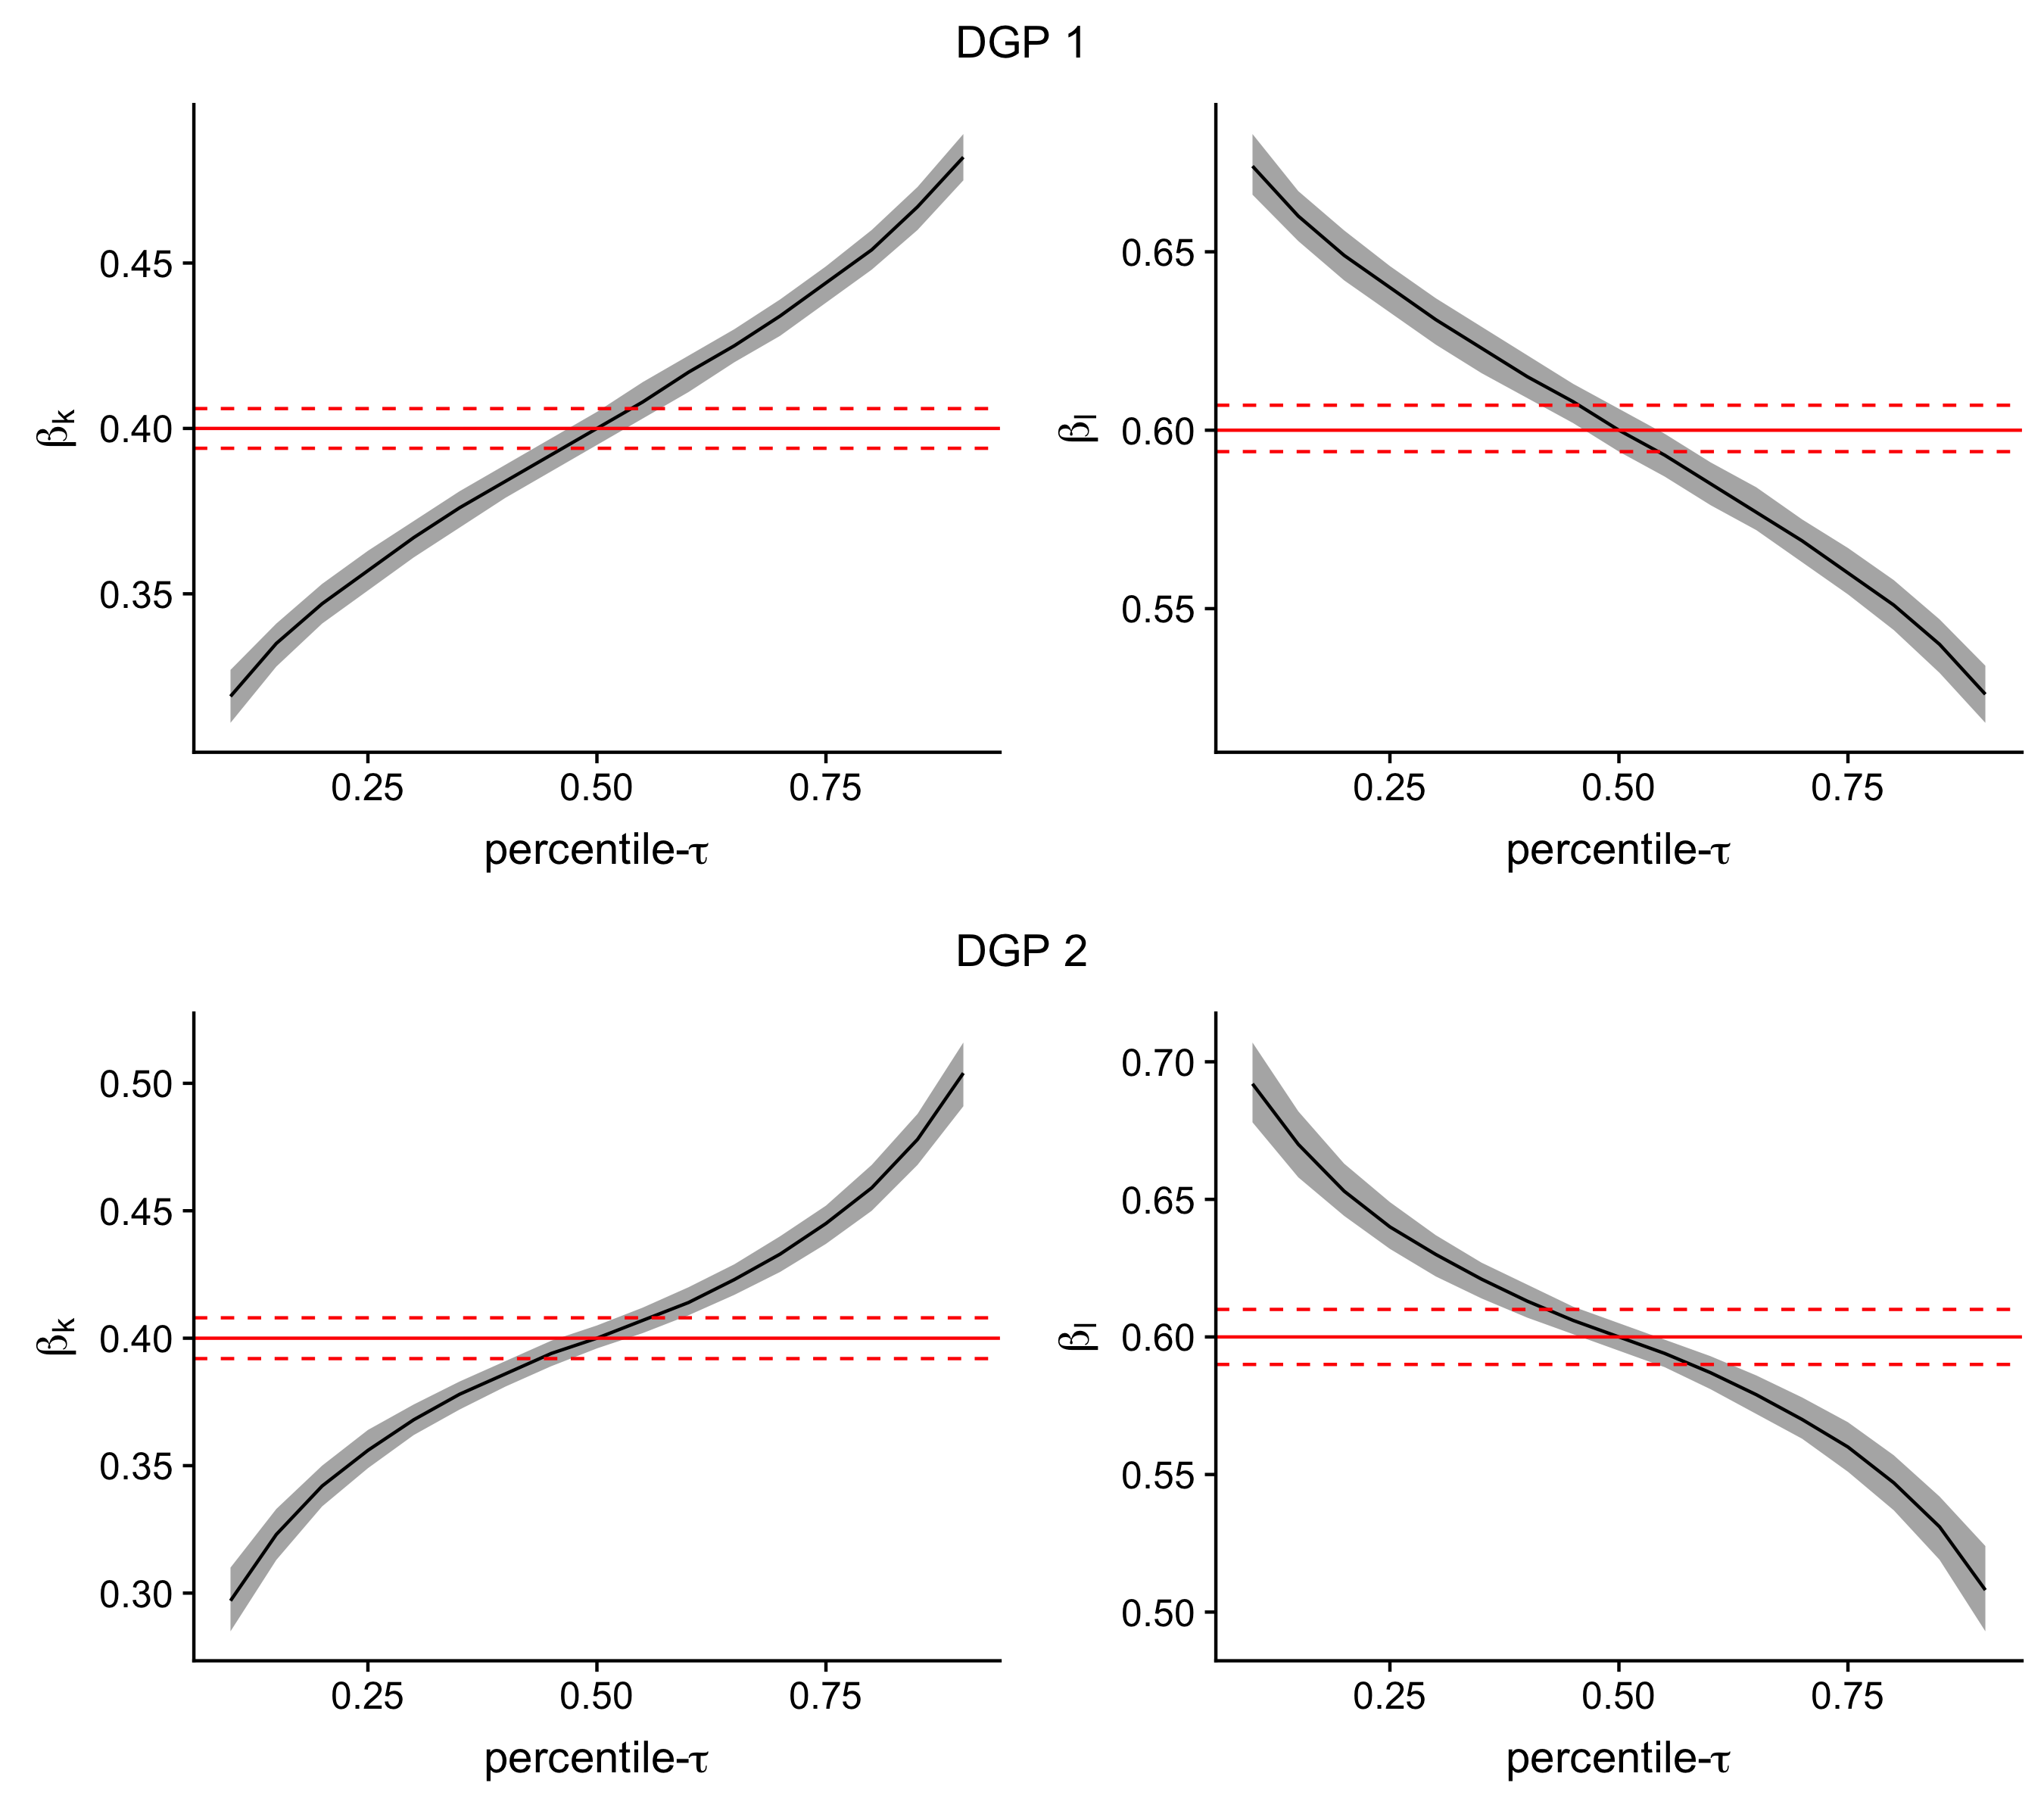
\includegraphics[width=11cm, height=9cm]{/Users/justindoty/Documents/Research/Dissertation/Production_QR_Proxy/Code/Monte_Carlo/LP_Coefficient_Plot.png}
\label{LP_coefficient_plot}
\end{figure}


\begin{figure}[H]
\centering
\caption{Simulated precision of  QLP estimators of $\beta_{k}(\tau)$ and $\beta_{l}(\tau)$s. Dotted line is LP estimator.}
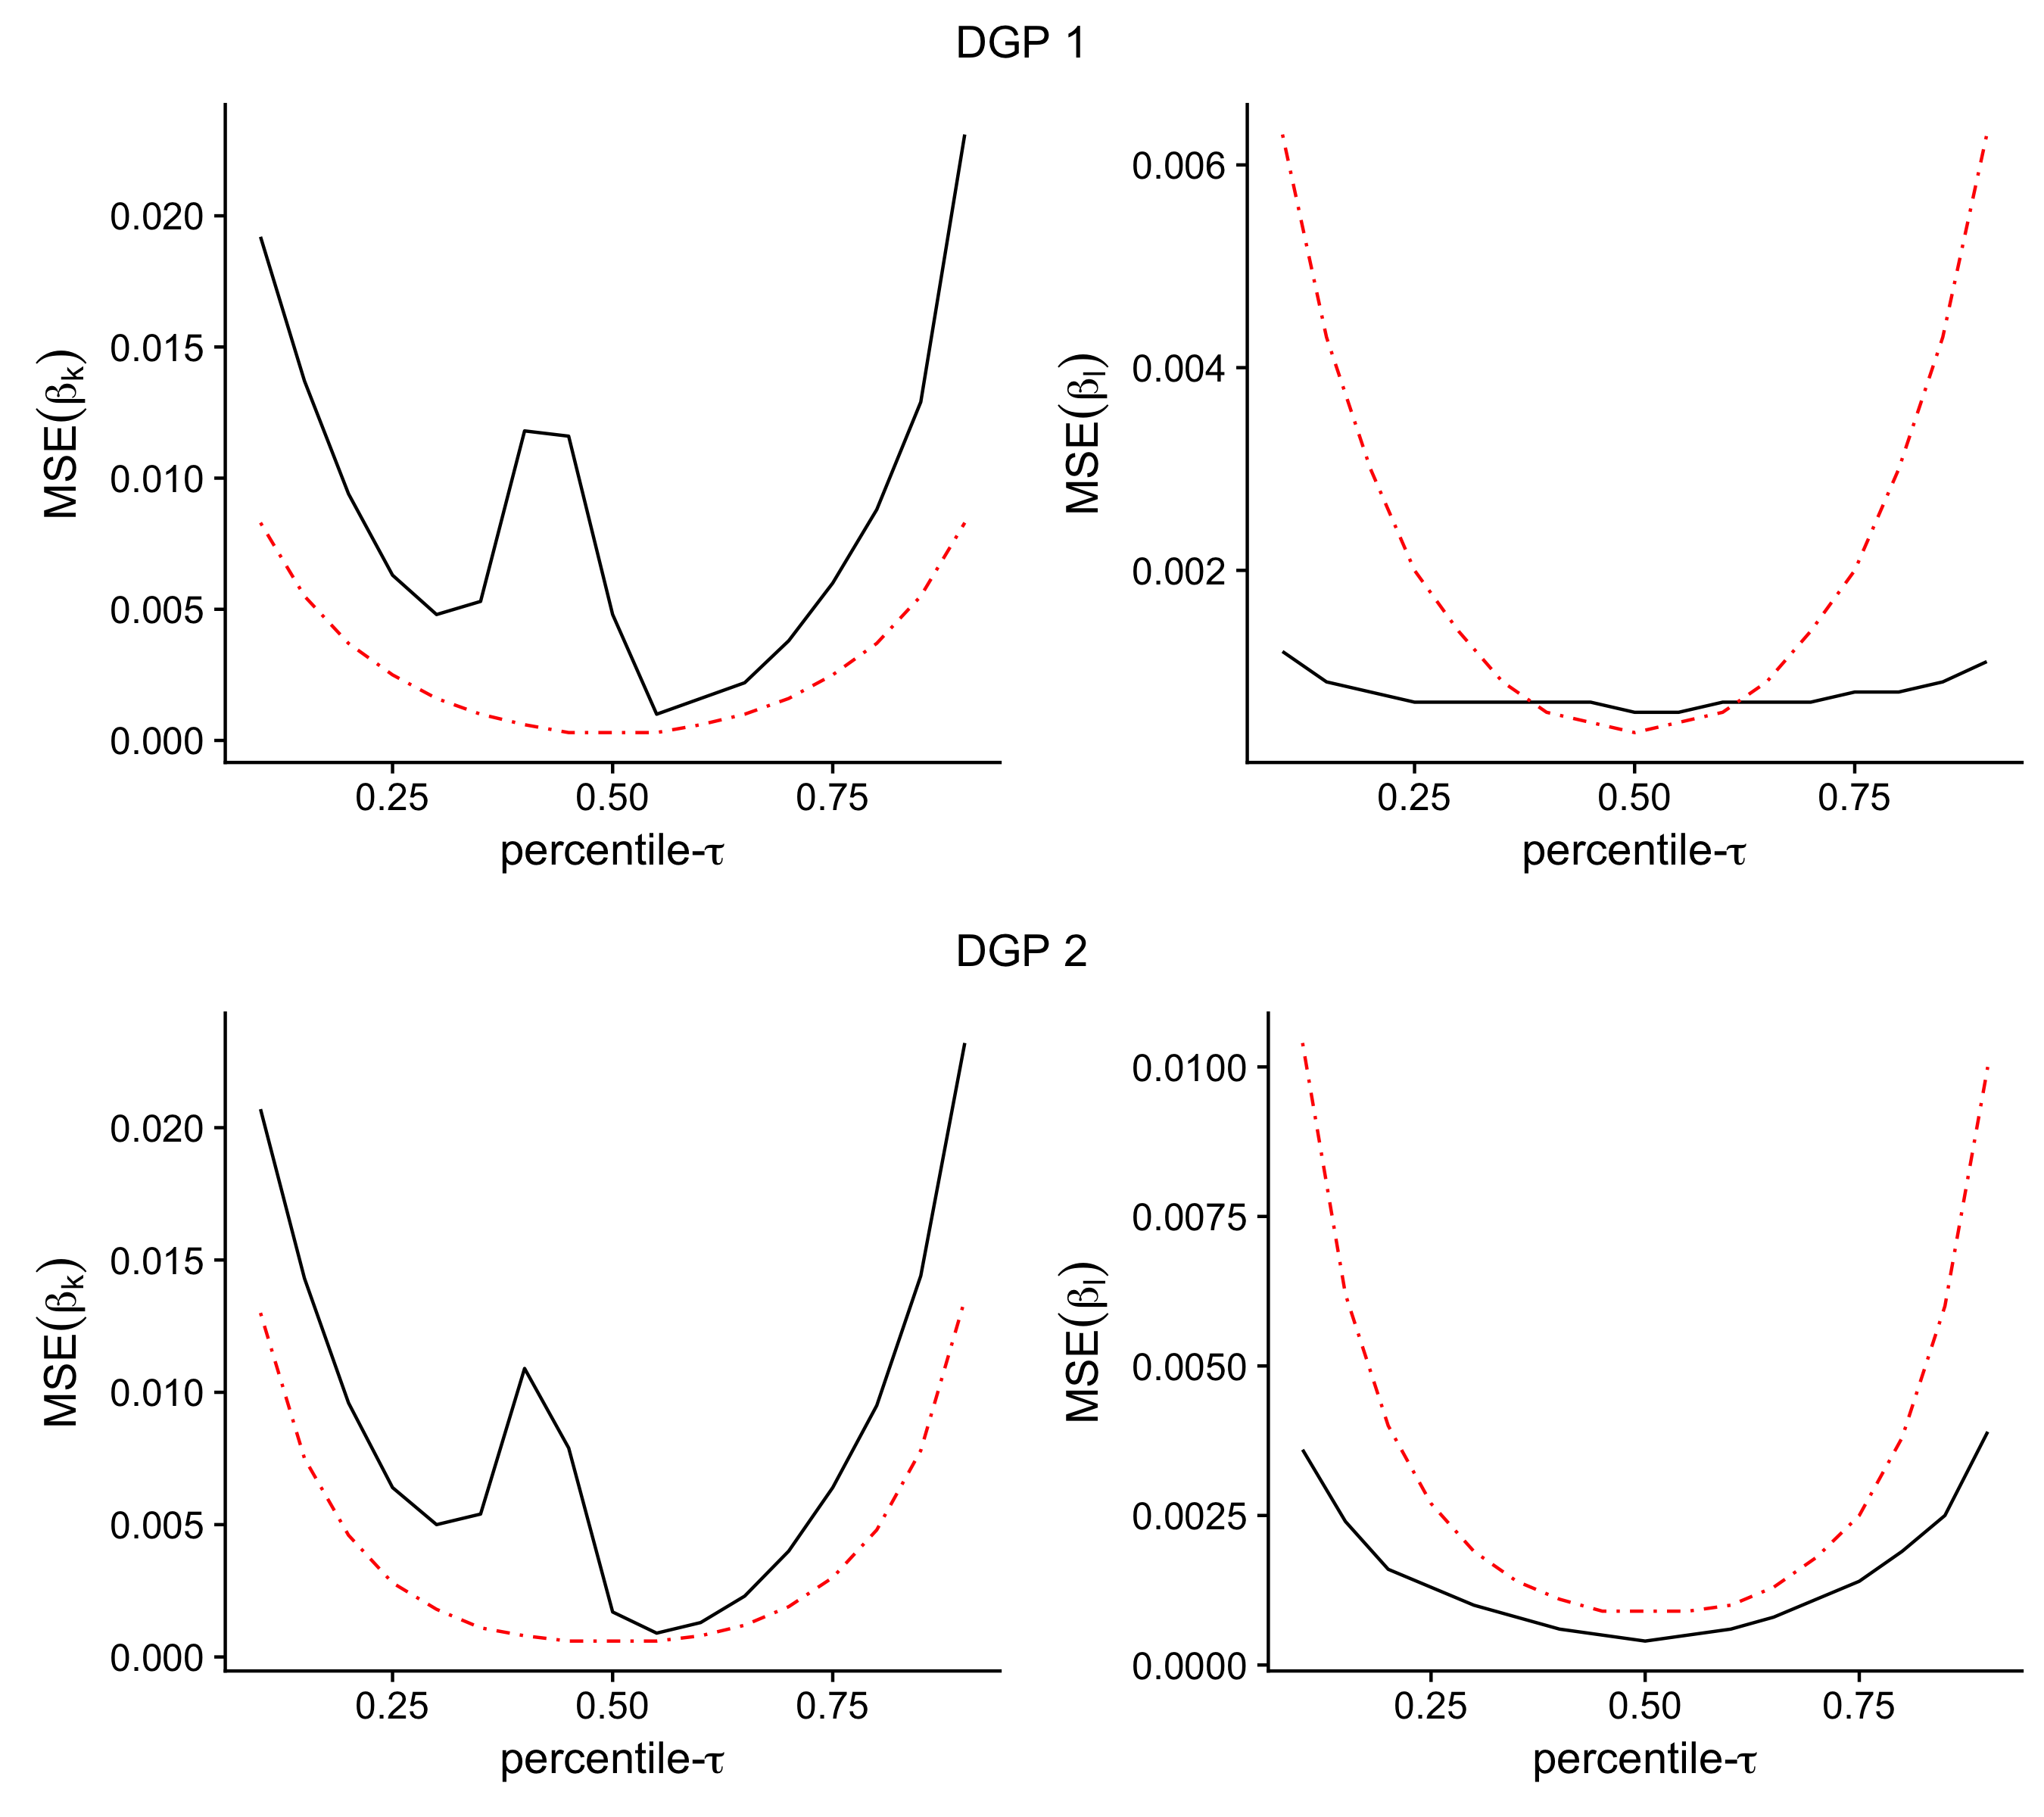
\includegraphics[width=11cm, height=9cm]{/Users/justindoty/Documents/Research/Dissertation/Production_QR_Proxy/Code/Monte_Carlo/LP_MSE_Plot.png}
\label{MSE_plot}
\end{figure}


The next figure summarizes distributional information from our Monte Carlo experiment. These simulation results show that our estimator has good finite-sample performance and does reasonably well at capturing firm heterogeneity across quantiles.

\begin{figure}[H]
\centering
\caption{LP Box Plots for estimated coefficients from 1000 replications of Monte Carlo}
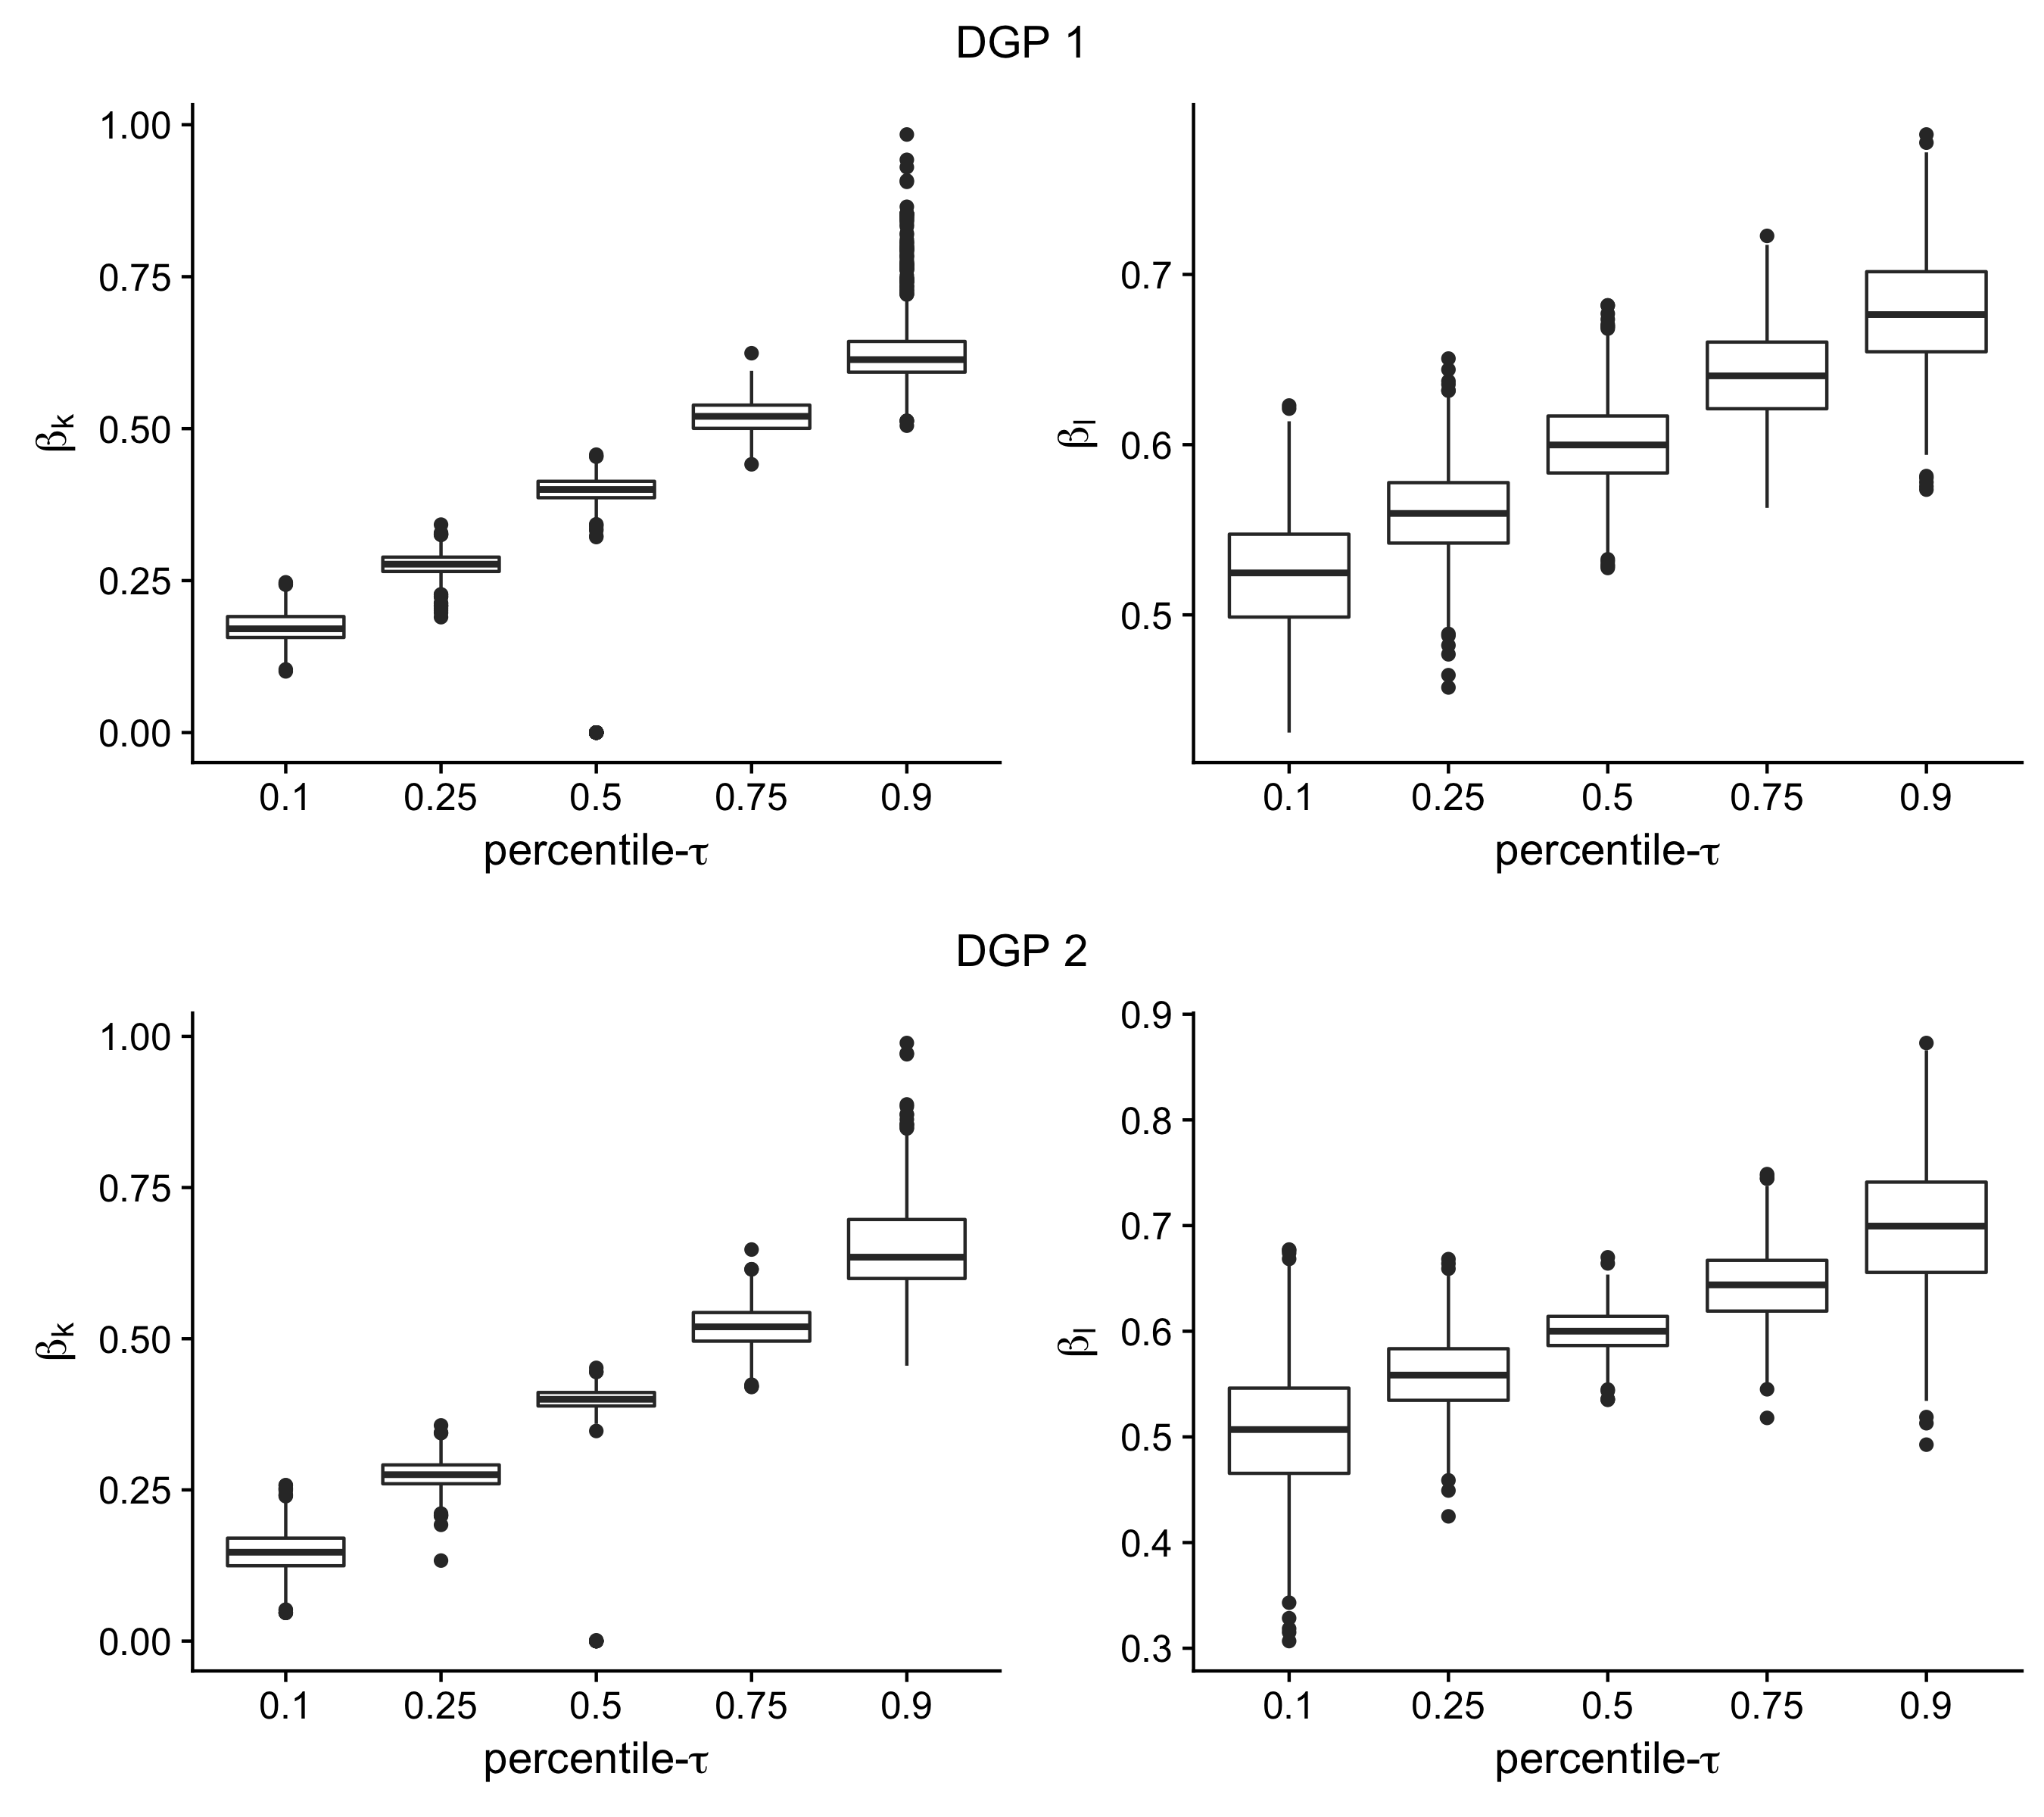
\includegraphics[width=12cm]{/Users/justindoty/Documents/Research/Dissertation/Production_QR_Proxy/Code/Monte_Carlo/QLP_Box_Plot.png}
\label{LP_Box Plot}
\end{figure}

\section{Application} \label{application}

\subsection{US Compustat}

% latex table generated in R 3.4.1 by xtable 1.8-2 package
% Fri Mar  5 12:36:22 2021
\begin{table}[H]
\centering
\begin{tabular}{ccccccc}
  \hline\hline Industry (NAICS code) &   & 1st Qu. & Median & 3rd Qu. & Mean & sd \\ 
  \hline
31 (Total=3271) & Output & 19.05 & 20.24 & 21.57 & 20.3 & 1.77 \\ 
   & Capital & 18.66 & 20.37 & 21.76 & 20.19 & 2.12 \\ 
   & Labor & 17.42 & 19.08 & 20.61 & 19.02 & 2.21 \\ 
   & Materials & 17.96 & 19.59 & 21.15 & 19.54 & 2.21 \\ 
  32 (Total=7207) & Output & 15.67 & 17.04 & 18.51 & 17.01 & 2.05 \\ 
   & Capital & 15.65 & 17.51 & 19.13 & 17.31 & 2.41 \\ 
   & Labor & 14.44 & 16.01 & 17.57 & 16.01 & 2.29 \\ 
   & Materials & 14.89 & 16.53 & 18.25 & 16.52 & 2.37 \\ 
  33 (Total=13978) & Output & 7.38 & 8.58 & 9.8 & 8.5 & 1.67 \\ 
   & Capital & 6.67 & 8.29 & 9.74 & 8.15 & 1.95 \\ 
   & Labor & 6.01 & 7.42 & 8.91 & 7.48 & 1.93 \\ 
   & Materials & 6.33 & 7.82 & 9.29 & 7.82 & 1.95 \\ 
  All (Total=24456) & Output & 18.58 & 19.78 & 21.23 & 19.85 & 1.79 \\ 
   & Capital & 18.14 & 19.86 & 21.26 & 19.67 & 2.16 \\ 
   & Labor & 16.98 & 18.59 & 20.13 & 18.56 & 2.17 \\ 
   & Materials & 17.49 & 19.12 & 20.66 & 19.06 & 2.2 \\ 
   \hline
\end{tabular}
\end{table}

% latex table generated in R 3.4.1 by xtable 1.8-2 package
% Wed Feb  3 20:38:50 2021
\begin{table}[ht]
\centering
\caption{Coefficient Estimates and Standard Errors for US Manufacturing Firms} 
\begin{tabular}{cccccccccc}
  \hline\hline & & \multicolumn{2}{c}{Capital}  & \multicolumn{2}{c}{Labor} & \multicolumn{2}{c}{Returns to Scale} & \multicolumn{2}{c}{Capital Intensity}\\ \cmidrule(lr){3-4} \cmidrule(lr){5-6} \cmidrule(lr){7-8} \cmidrule(lr){9-10}NAICS & $\tau$ & Coef. & s.e & Coef. & s.e & Coef. & s.e & Coef. & s.e \\ 
  \hline
31 & 0.10 & 0.563 & 0.0764 & 0.607 & 0.0311 & 1.170 & 0.0816 & 0.928 & 0.1368 \\ 
   & 0.25 & 0.113 & 0.1476 & 0.543 & 0.0372 & 0.656 & 0.1478 & 0.208 & 0.2740 \\ 
   & 0.50 & 0.122 & 0.1388 & 0.464 & 0.0354 & 0.586 & 0.1468 & 0.263 & 0.2994 \\ 
   & 0.90 & 0.147 & 0.1359 & 0.456 & 0.0452 & 0.603 & 0.1452 & 0.322 & 0.3178 \\ 
  32 & 0.10 & 0.081 & 0.1043 & 0.654 & 0.0497 & 0.735 & 0.0816 & 0.123 & 0.1594 \\ 
   & 0.25 & 0.092 & 0.0577 & 0.605 & 0.0332 & 0.697 & 0.0615 & 0.152 & 0.0992 \\ 
   & 0.50 & 0.102 & 0.0624 & 0.561 & 0.0264 & 0.663 & 0.0666 & 0.182 & 0.1130 \\ 
   & 0.90 & 0.124 & 0.0647 & 0.526 & 0.0307 & 0.649 & 0.0725 & 0.235 & 0.1341 \\ 
  33 & 0.10 & 0.014 & 0.0488 & 0.210 & 0.0598 & 0.223 & 0.0728 & 0.066 & 0.3861 \\ 
   & 0.25 & 0.043 & 0.0499 & 0.354 & 0.0432 & 0.397 & 0.0618 & 0.121 & 0.1664 \\ 
   & 0.50 & 0.064 & 0.0478 & 0.439 & 0.0304 & 0.503 & 0.0541 & 0.146 & 0.1164 \\ 
   & 0.90 & 0.098 & 0.0476 & 0.446 & 0.0287 & 0.544 & 0.0524 & 0.220 & 0.1133 \\ 
  All & 0.10 & 0.049 & 0.0410 & 0.363 & 0.0420 & 0.412 & 0.0547 & 0.135 & 0.1558 \\ 
   & 0.25 & 0.070 & 0.0373 & 0.411 & 0.0257 & 0.481 & 0.0437 & 0.169 & 0.1017 \\ 
   & 0.50 & 0.087 & 0.0322 & 0.470 & 0.0201 & 0.558 & 0.0365 & 0.186 & 0.0754 \\ 
   & 0.90 & 0.117 & 0.0322 & 0.474 & 0.0179 & 0.591 & 0.0352 & 0.247 & 0.0748 \\ 
   \hline
\end{tabular}
\end{table}


\begin{figure}[H]
\centering
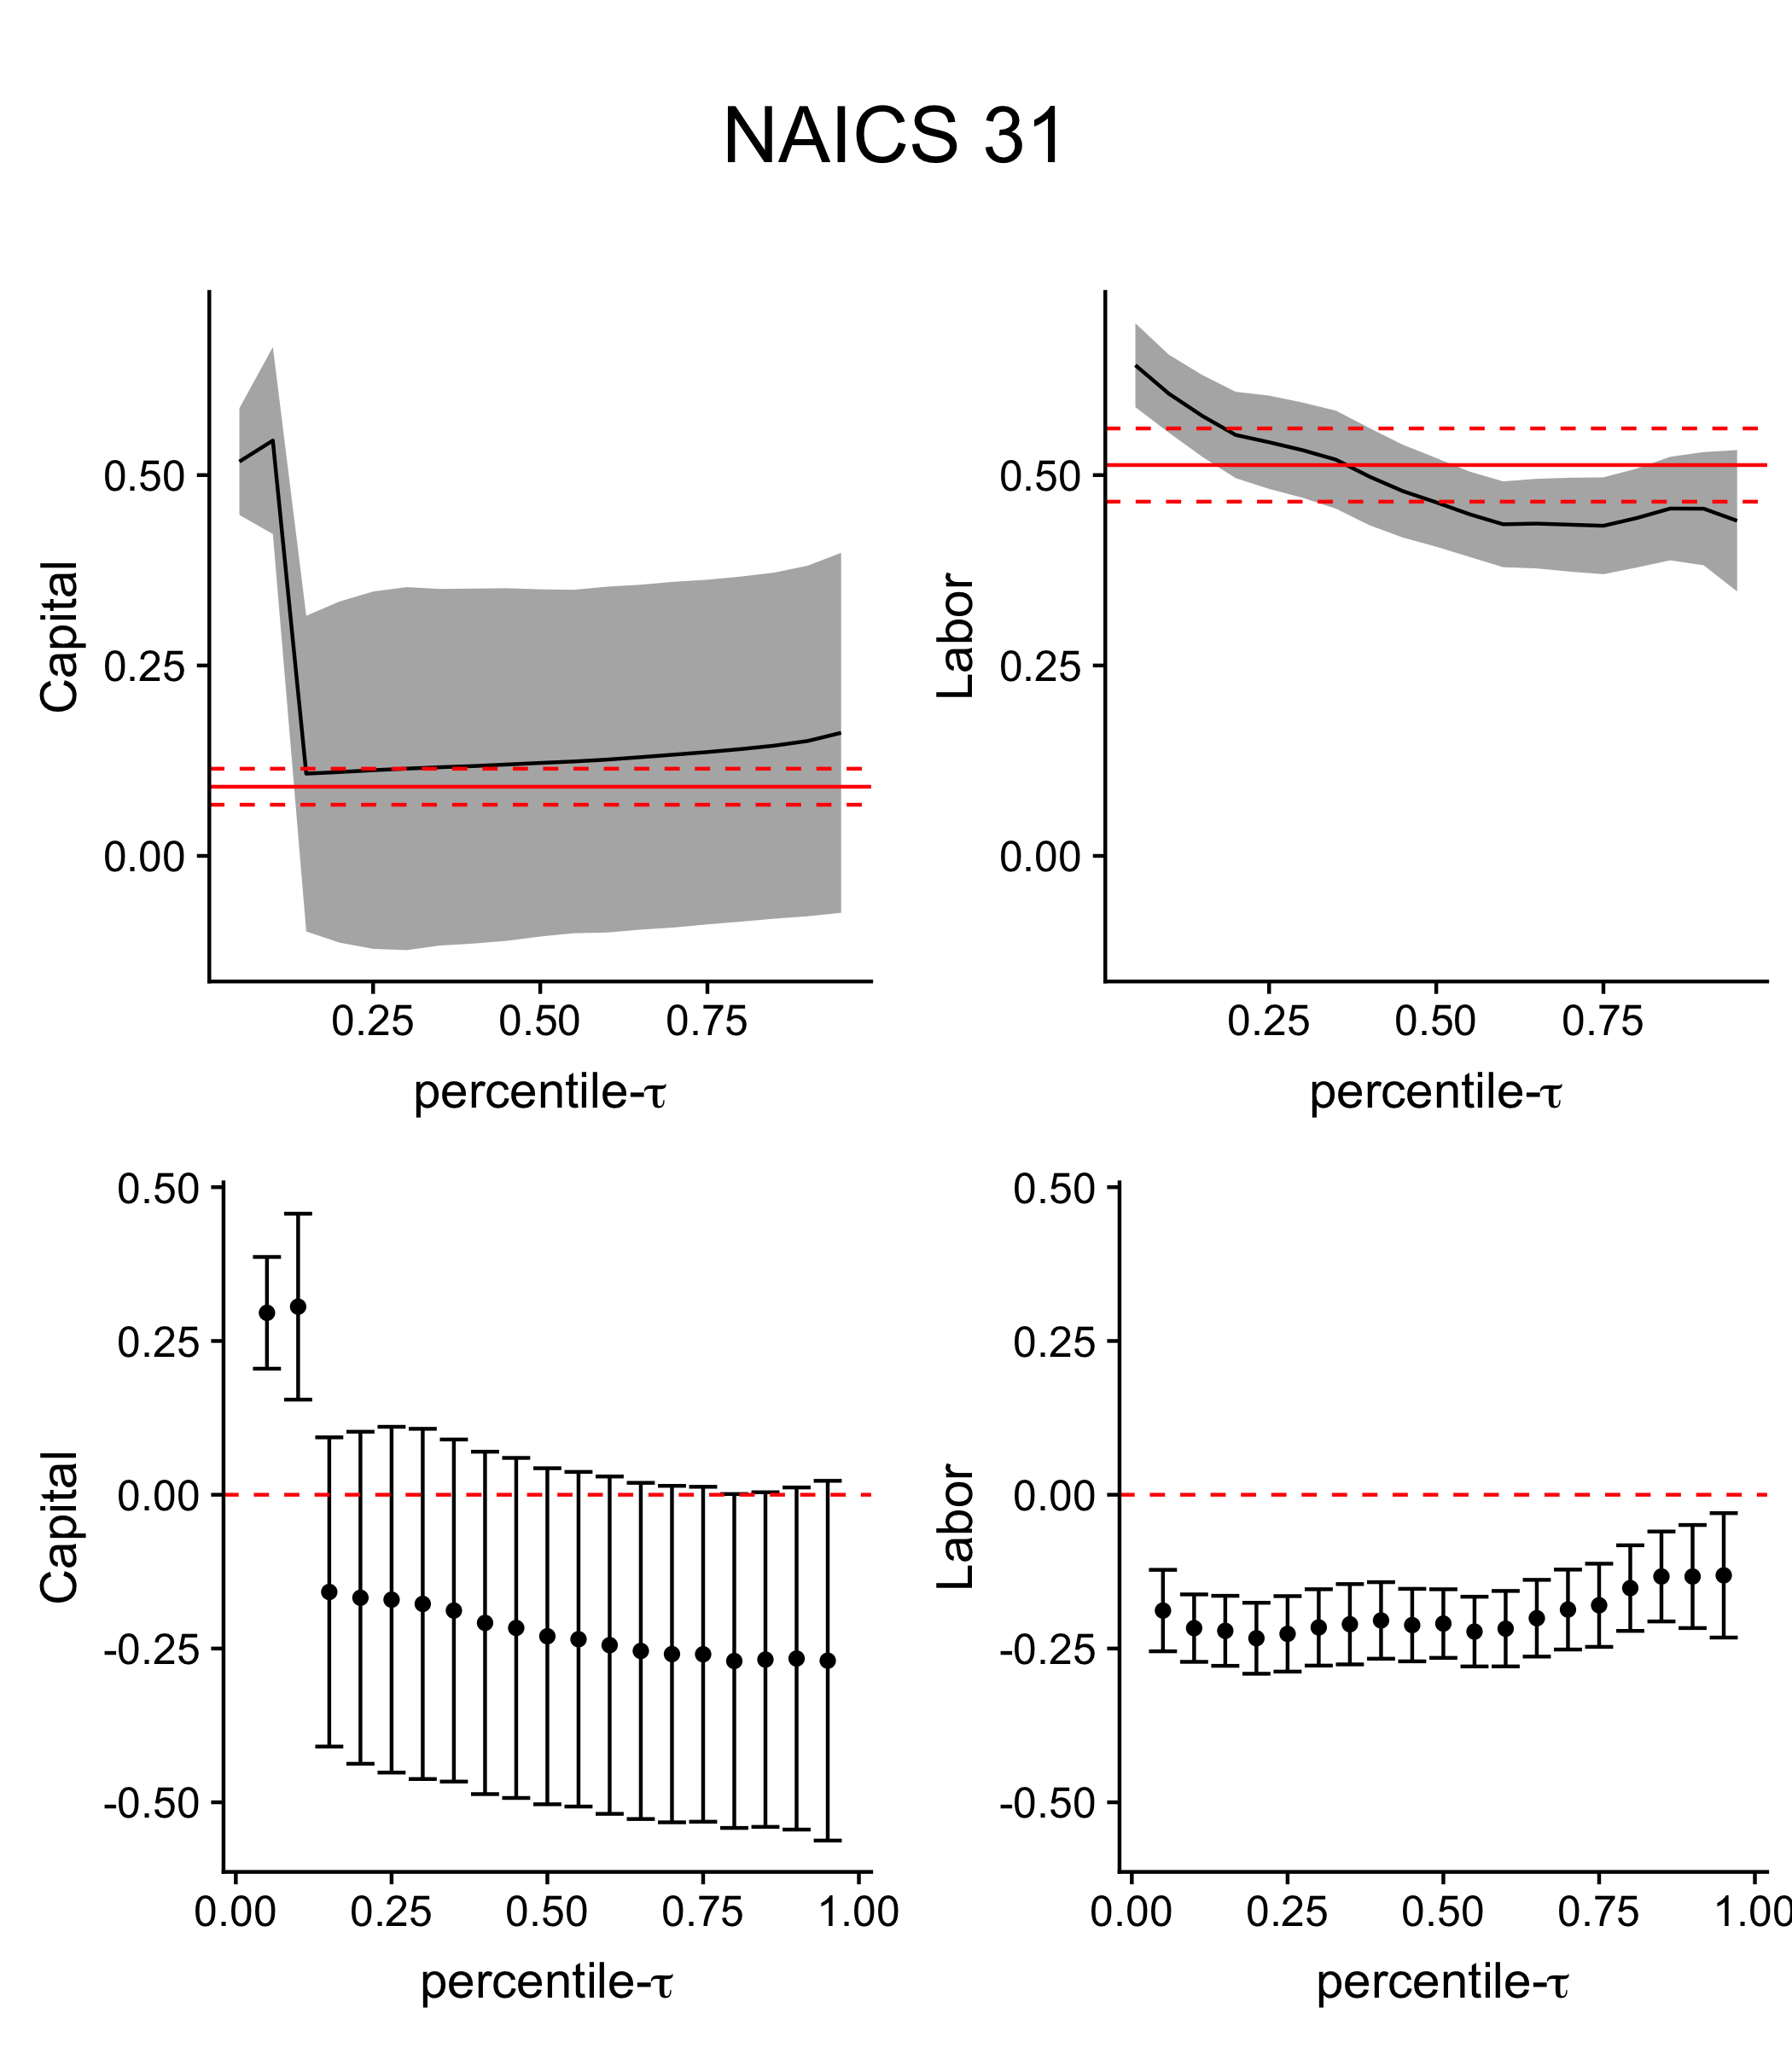
\includegraphics[width=12cm]{/Users/justindoty/Documents/Research/Dissertation/Production_QR_Proxy/Code/Empirical/US/Plots/Coef_Plot_NAICS_31.png}
\caption{Estimated values of production function coefficients and their 90\% confidence interval. The plots on the LHS are the QLP and LP estimates. The plots on the RHS are quantile regression and OLS estimates.}
\end{figure}

\begin{figure}[H]
\centering
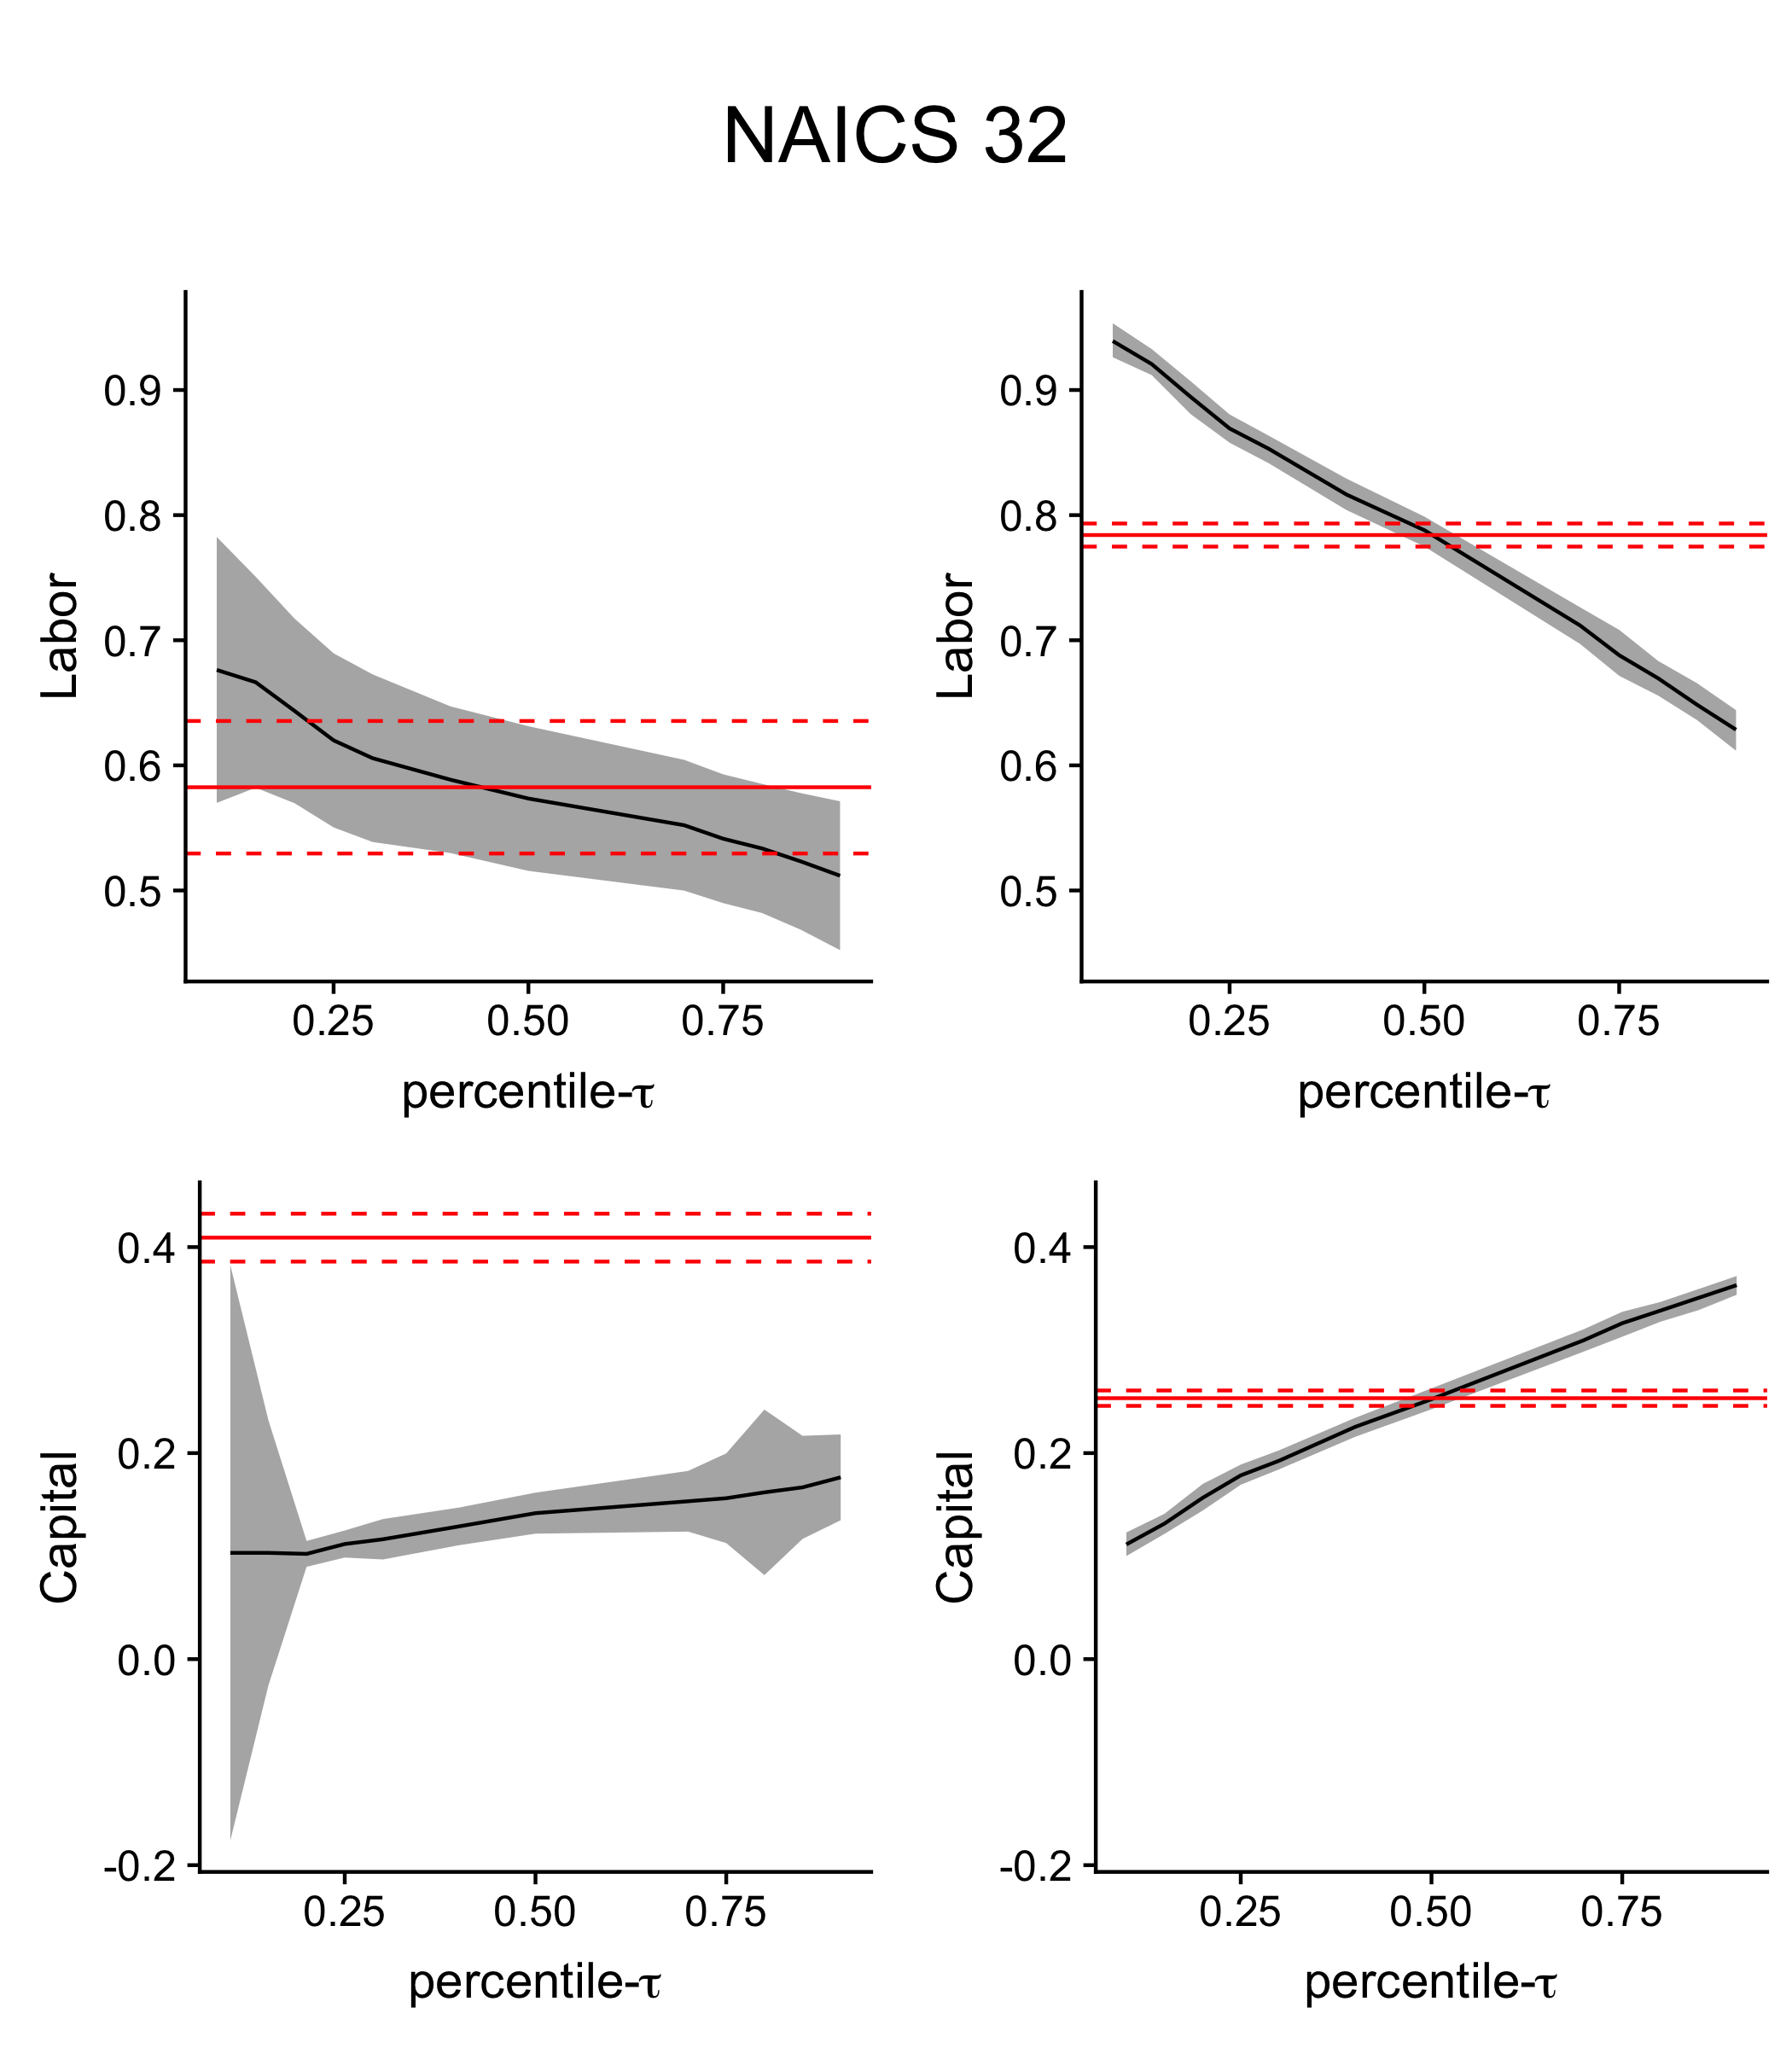
\includegraphics[width=12cm]{/Users/justindoty/Documents/Research/Dissertation/Production_QR_Proxy/Code/Empirical/US/Plots/Coef_Plot_NAICS_32.png}
\caption{Estimated values of production function coefficients and their 90\% confidence interval. The plots on the LHS are the QLP and LP estimates. The plots on the RHS are quantile regression and OLS estimates.}
\end{figure}

\begin{figure}[H]
\centering
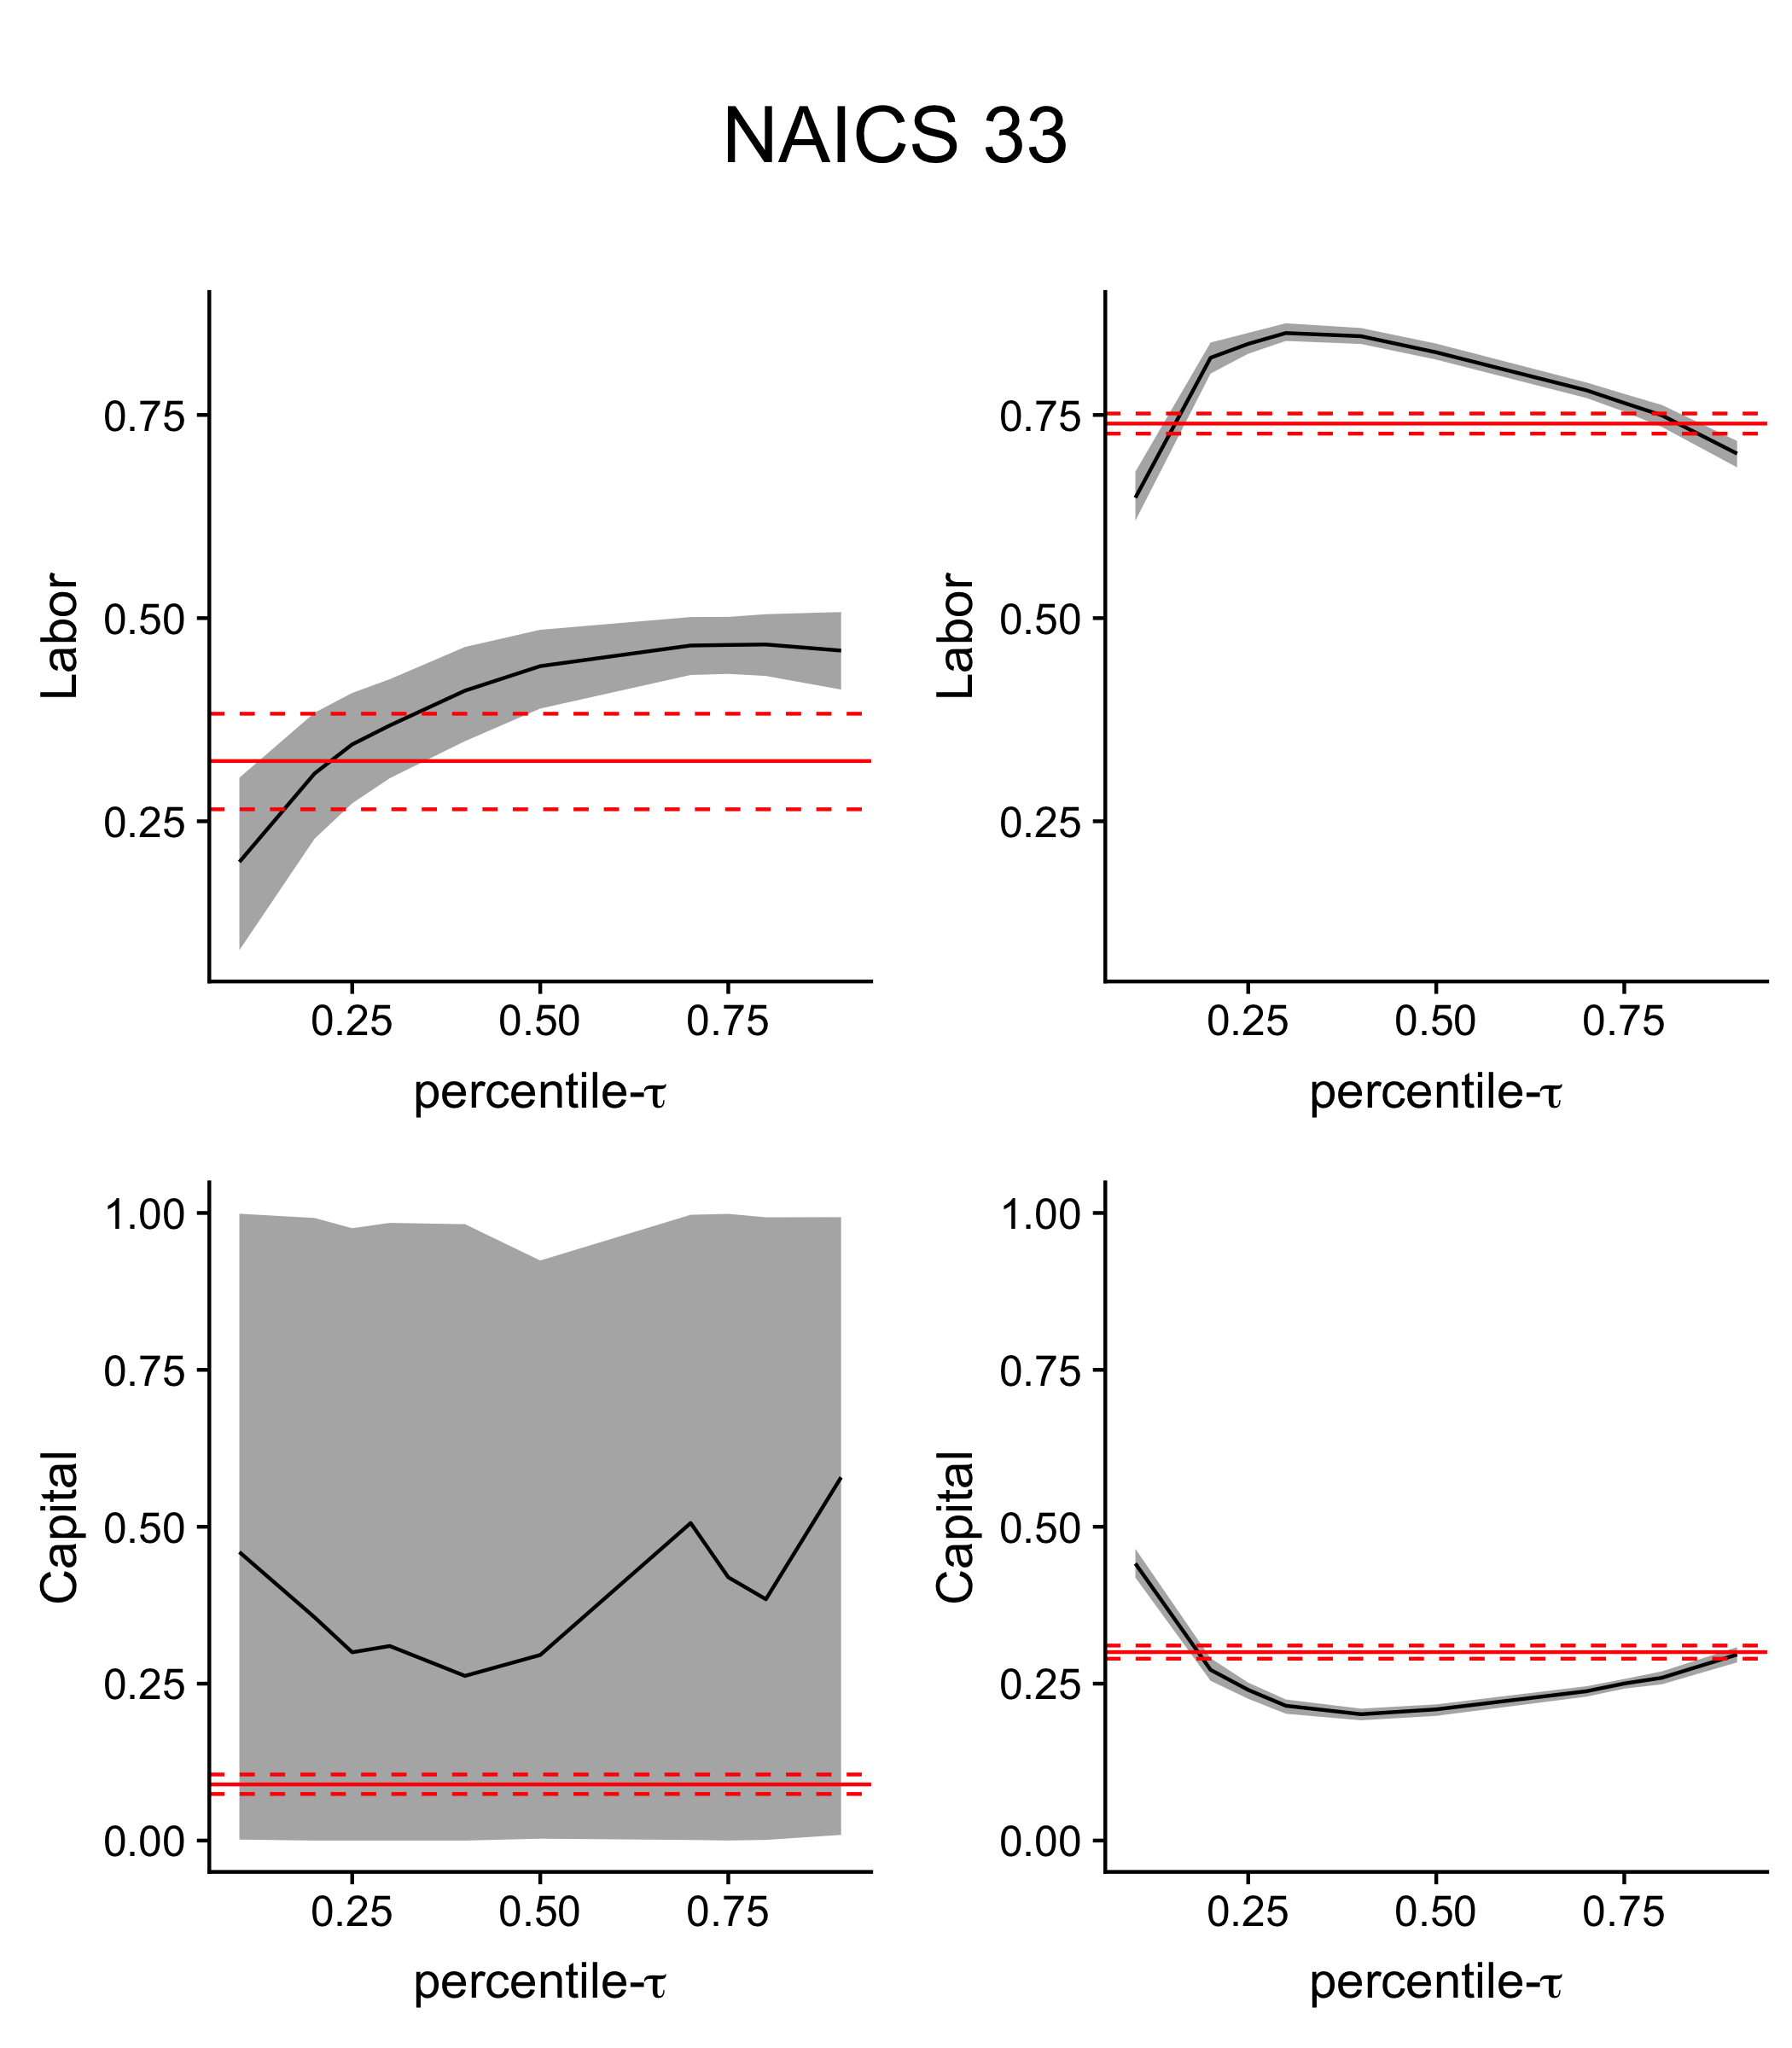
\includegraphics[width=12cm]{/Users/justindoty/Documents/Research/Dissertation/Production_QR_Proxy/Code/Empirical/US/Plots/Coef_Plot_NAICS_33.png}
\caption{Estimated values of production function coefficients and their 90\% confidence interval. The plots on the LHS are the QLP and LP estimates. The plots on the RHS are quantile regression and OLS estimates.}
\end{figure}

\begin{figure}[H]
\centering
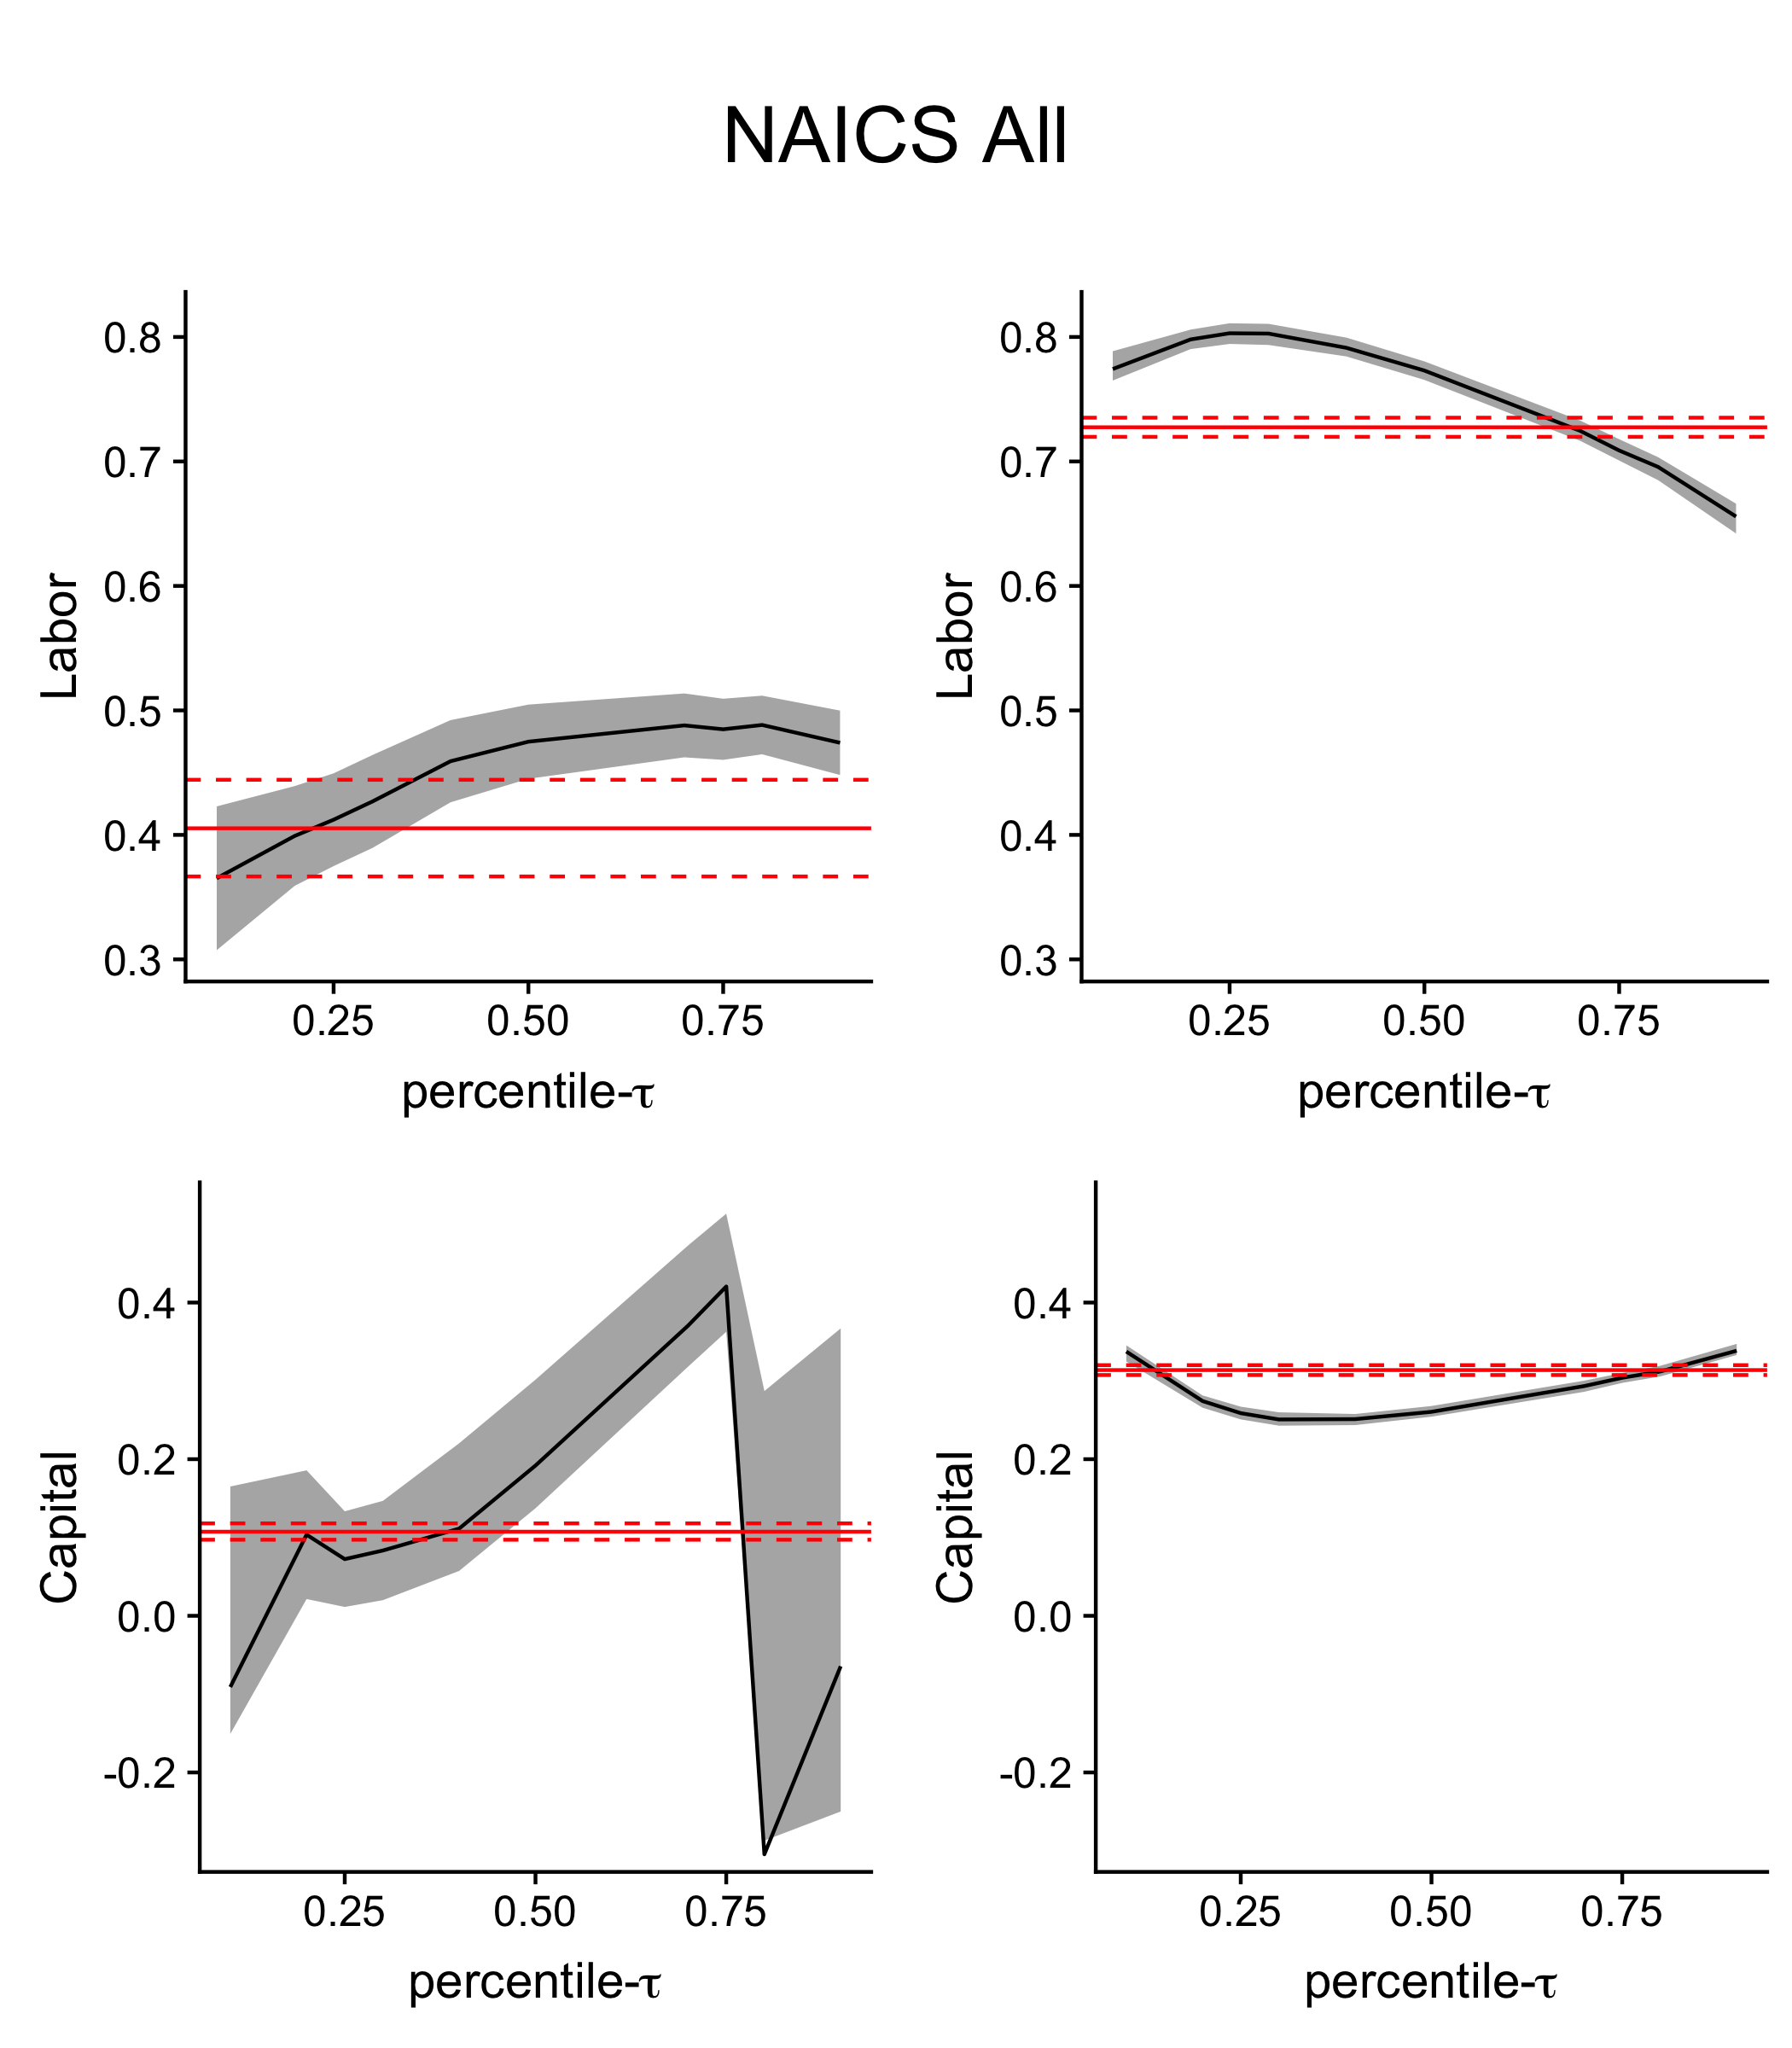
\includegraphics[width=12cm]{/Users/justindoty/Documents/Research/Dissertation/Production_QR_Proxy/Code/Empirical/US/Plots/Coef_Plot_NAICS_All.png}
\caption{Estimated values of production function coeficients and their 90\% confidence interval. The plots on the LHS are the QLP and LP estimates. The plots on the RHS are quantile regression and OLS estimates.}
\end{figure}

\begin{figure}[H]
\centering
\includegraphics[width=12cm]{/Users/justindoty/Documents/Research/Dissertation/Production_QR_Proxy/Code/Empirical/US/Plots/TFP_Plot.png}
\caption{Estimated average TFP over time for the US. Base productivity in 1961 is set to 100.}
\end{figure}

\begin{figure}[H]
\centering
\includegraphics[width=12cm]{/Users/justindoty/Documents/Research/Dissertation/Production_QR_Proxy/Code/Empirical/US/Plots/Q3Q1_Grid_plot.png}
\caption{Estimated 75/25 productivity dipersion ratio and their 90\% confidence interval by industry.}
\end{figure}

\begin{figure}[H]
\centering
\includegraphics[width=12cm]{/Users/justindoty/Documents/Research/Dissertation/Production_QR_Proxy/Code/Empirical/US/Plots/Q9Q1_Grid_plot.png}
\caption{Estimated 90/10 productivity dipersion ratio and their 90\% confidence interval by industry.}
\end{figure}

\begin{figure}[H]
\centering
\includegraphics[width=12cm]{/Users/justindoty/Documents/Research/Dissertation/Production_QR_Proxy/Code/Empirical/US/Plots/Q95Q05_Grid_plot.png}
\caption{Estimated 95/5 productivity dipersion ratio and their 90\% confidence interval by industry.}
\end{figure}

\begin{figure}[H]
\centering
\includegraphics[width=12cm]{/Users/justindoty/Documents/Research/Dissertation/Production_QR_Proxy/Code/Empirical/US/Plots/Time_Plot.png}
\caption{Estimated values of production function coefficients over time estimated at 5 year intervals}
\end{figure}


%----------------------------------------------------------------------------------------

\subsection{Chilean Manufacturing}

% latex table generated in R 3.4.1 by xtable 1.8-2 package
% Wed Jan  6 11:45:58 2021
\begin{table}[H]
\centering
\caption{Summary Statistics (in logs) for Chile Manufacturing Data} 
\begin{tabular}{ccccccc}
  \hline\hline Industry (ISIC code) &   & 1st Qu. & Median & 3rd Qu. & Mean & sd \\ 
  \hline
311 (Total=13838) & Output & 10.21 & 10.84 & 12.22 & 11.36 & 1.58 \\ 
   & Capital & 10.56 & 11.4 & 12.4 & 11.52 & 1.37 \\ 
   & Labor & 10.49 & 11.4 & 12.54 & 11.53 & 1.43 \\ 
   & Materials & 10.38 & 11.28 & 12.53 & 11.56 & 1.6 \\ 
  381 (Total=4311) & Output & 6.69 & 7.66 & 9.06 & 8.02 & 1.98 \\ 
   & Capital & 7.52 & 8.51 & 9.7 & 8.65 & 1.68 \\ 
   & Labor & 7.21 & 8.34 & 9.56 & 8.4 & 1.72 \\ 
   & Materials & 7.22 & 8.35 & 9.72 & 8.54 & 1.92 \\ 
  321 (Total=4302) & Output & 2.77 & 3.22 & 3.91 & 3.49 & 0.99 \\ 
   & Capital & 2.89 & 3.47 & 4.22 & 3.71 & 1.08 \\ 
   & Labor & 2.94 & 3.48 & 4.37 & 3.69 & 0.95 \\ 
   & Materials & 2.89 & 3.43 & 4.28 & 3.67 & 1.02 \\ 
  All (Total=51567) & Output & 9.84 & 10.46 & 11.81 & 10.94 & 1.56 \\ 
   & Capital & 9.91 & 10.75 & 11.79 & 10.86 & 1.41 \\ 
   & Labor & 9.68 & 10.62 & 11.75 & 10.73 & 1.48 \\ 
   & Materials & 9.81 & 10.68 & 11.89 & 10.93 & 1.62 \\ 
   \hline
\end{tabular}
\end{table}

% latex table generated in R 3.4.1 by xtable 1.8-2 package
% Thu Feb  4 15:46:40 2021
\begin{table}[ht]
\centering
\caption{Coefficient Estimates and Standard Errors for Chilean Manufacturing Firms} 
\begin{tabular}{cccccccccc}
  \hline\hline & & \multicolumn{2}{c}{Capital}  & \multicolumn{2}{c}{Labor} & \multicolumn{2}{c}{Returns to Scale} & \multicolumn{2}{c}{Capital Intensity}\\ \cmidrule(lr){3-4} \cmidrule(lr){5-6} \cmidrule(lr){7-8} \cmidrule(lr){9-10}ISIC & $\tau$ & Coef. & s.e & Coef. & s.e & Coef. & s.e & Coef. & s.e \\ 
  \hline
311 & 0.10 & 0.179 & 0.0248 & 0.380 & 0.0523 & 0.559 & 0.0486 & 0.470 & 0.1071 \\ 
   & 0.25 & 0.254 & 0.0246 & 0.380 & 0.0351 & 0.635 & 0.0357 & 0.668 & 0.0929 \\ 
   & 0.50 & 0.309 & 0.0232 & 0.423 & 0.0263 & 0.731 & 0.0310 & 0.730 & 0.0807 \\ 
   & 0.90 & 0.412 & 0.0248 & 0.444 & 0.0364 & 0.857 & 0.0354 & 0.927 & 0.1114 \\ 
  381 & 0.10 & 0.250 & 0.0485 & 0.774 & 0.0800 & 1.024 & 0.0570 & 0.322 & 0.1019 \\ 
   & 0.25 & 0.362 & 0.0393 & 0.649 & 0.0533 & 1.011 & 0.0460 & 0.558 & 0.1029 \\ 
   & 0.50 & 0.425 & 0.0379 & 0.606 & 0.0431 & 1.030 & 0.0405 & 0.701 & 0.1175 \\ 
   & 0.90 & 0.568 & 0.0439 & 0.503 & 0.0523 & 1.071 & 0.0450 & 1.129 & 0.2155 \\ 
  321 & 0.10 & 0.349 & 0.0571 & 0.677 & 0.0847 & 1.026 & 0.0559 & 0.516 & 0.1375 \\ 
   & 0.25 & 0.466 & 0.0478 & 0.564 & 0.0614 & 1.030 & 0.0455 & 0.827 & 0.1424 \\ 
   & 0.50 & 0.518 & 0.0440 & 0.553 & 0.0484 & 1.071 & 0.0408 & 0.937 & 0.1403 \\ 
   & 0.90 & 0.643 & 0.0481 & 0.538 & 0.0502 & 1.180 & 0.0440 & 1.195 & 0.1932 \\ 
  All & 0.10 & 0.532 & 0.0166 & 0.522 & 0.0267 & 1.055 & 0.0171 & 1.020 & 0.0799 \\ 
   & 0.25 & 0.618 & 0.0139 & 0.487 & 0.0197 & 1.105 & 0.0143 & 1.268 & 0.0725 \\ 
   & 0.50 & 0.689 & 0.0128 & 0.457 & 0.0158 & 1.145 & 0.0127 & 1.508 & 0.0720 \\ 
   & 0.90 & 0.499 & 0.0136 & 0.391 & 0.0211 & 0.891 & 0.0183 & 1.275 & 0.0935 \\ 
   \hline
\end{tabular}
\end{table}


\begin{figure}[H]
\centering
\includegraphics[width=12cm]{/Users/justindoty/Documents/Research/Dissertation/Production_QR_Proxy/Code/Empirical/Chile/Plots/Coef_Plot_ISIC_311.png}
\caption{Estimated values of production function coefficients and their 90\% confidence interval. The plots on the LHS are the QLP and LP estimates. The plots on the RHS are quantile regression and OLS estimates.}
\end{figure}

\begin{figure}[H]
\centering
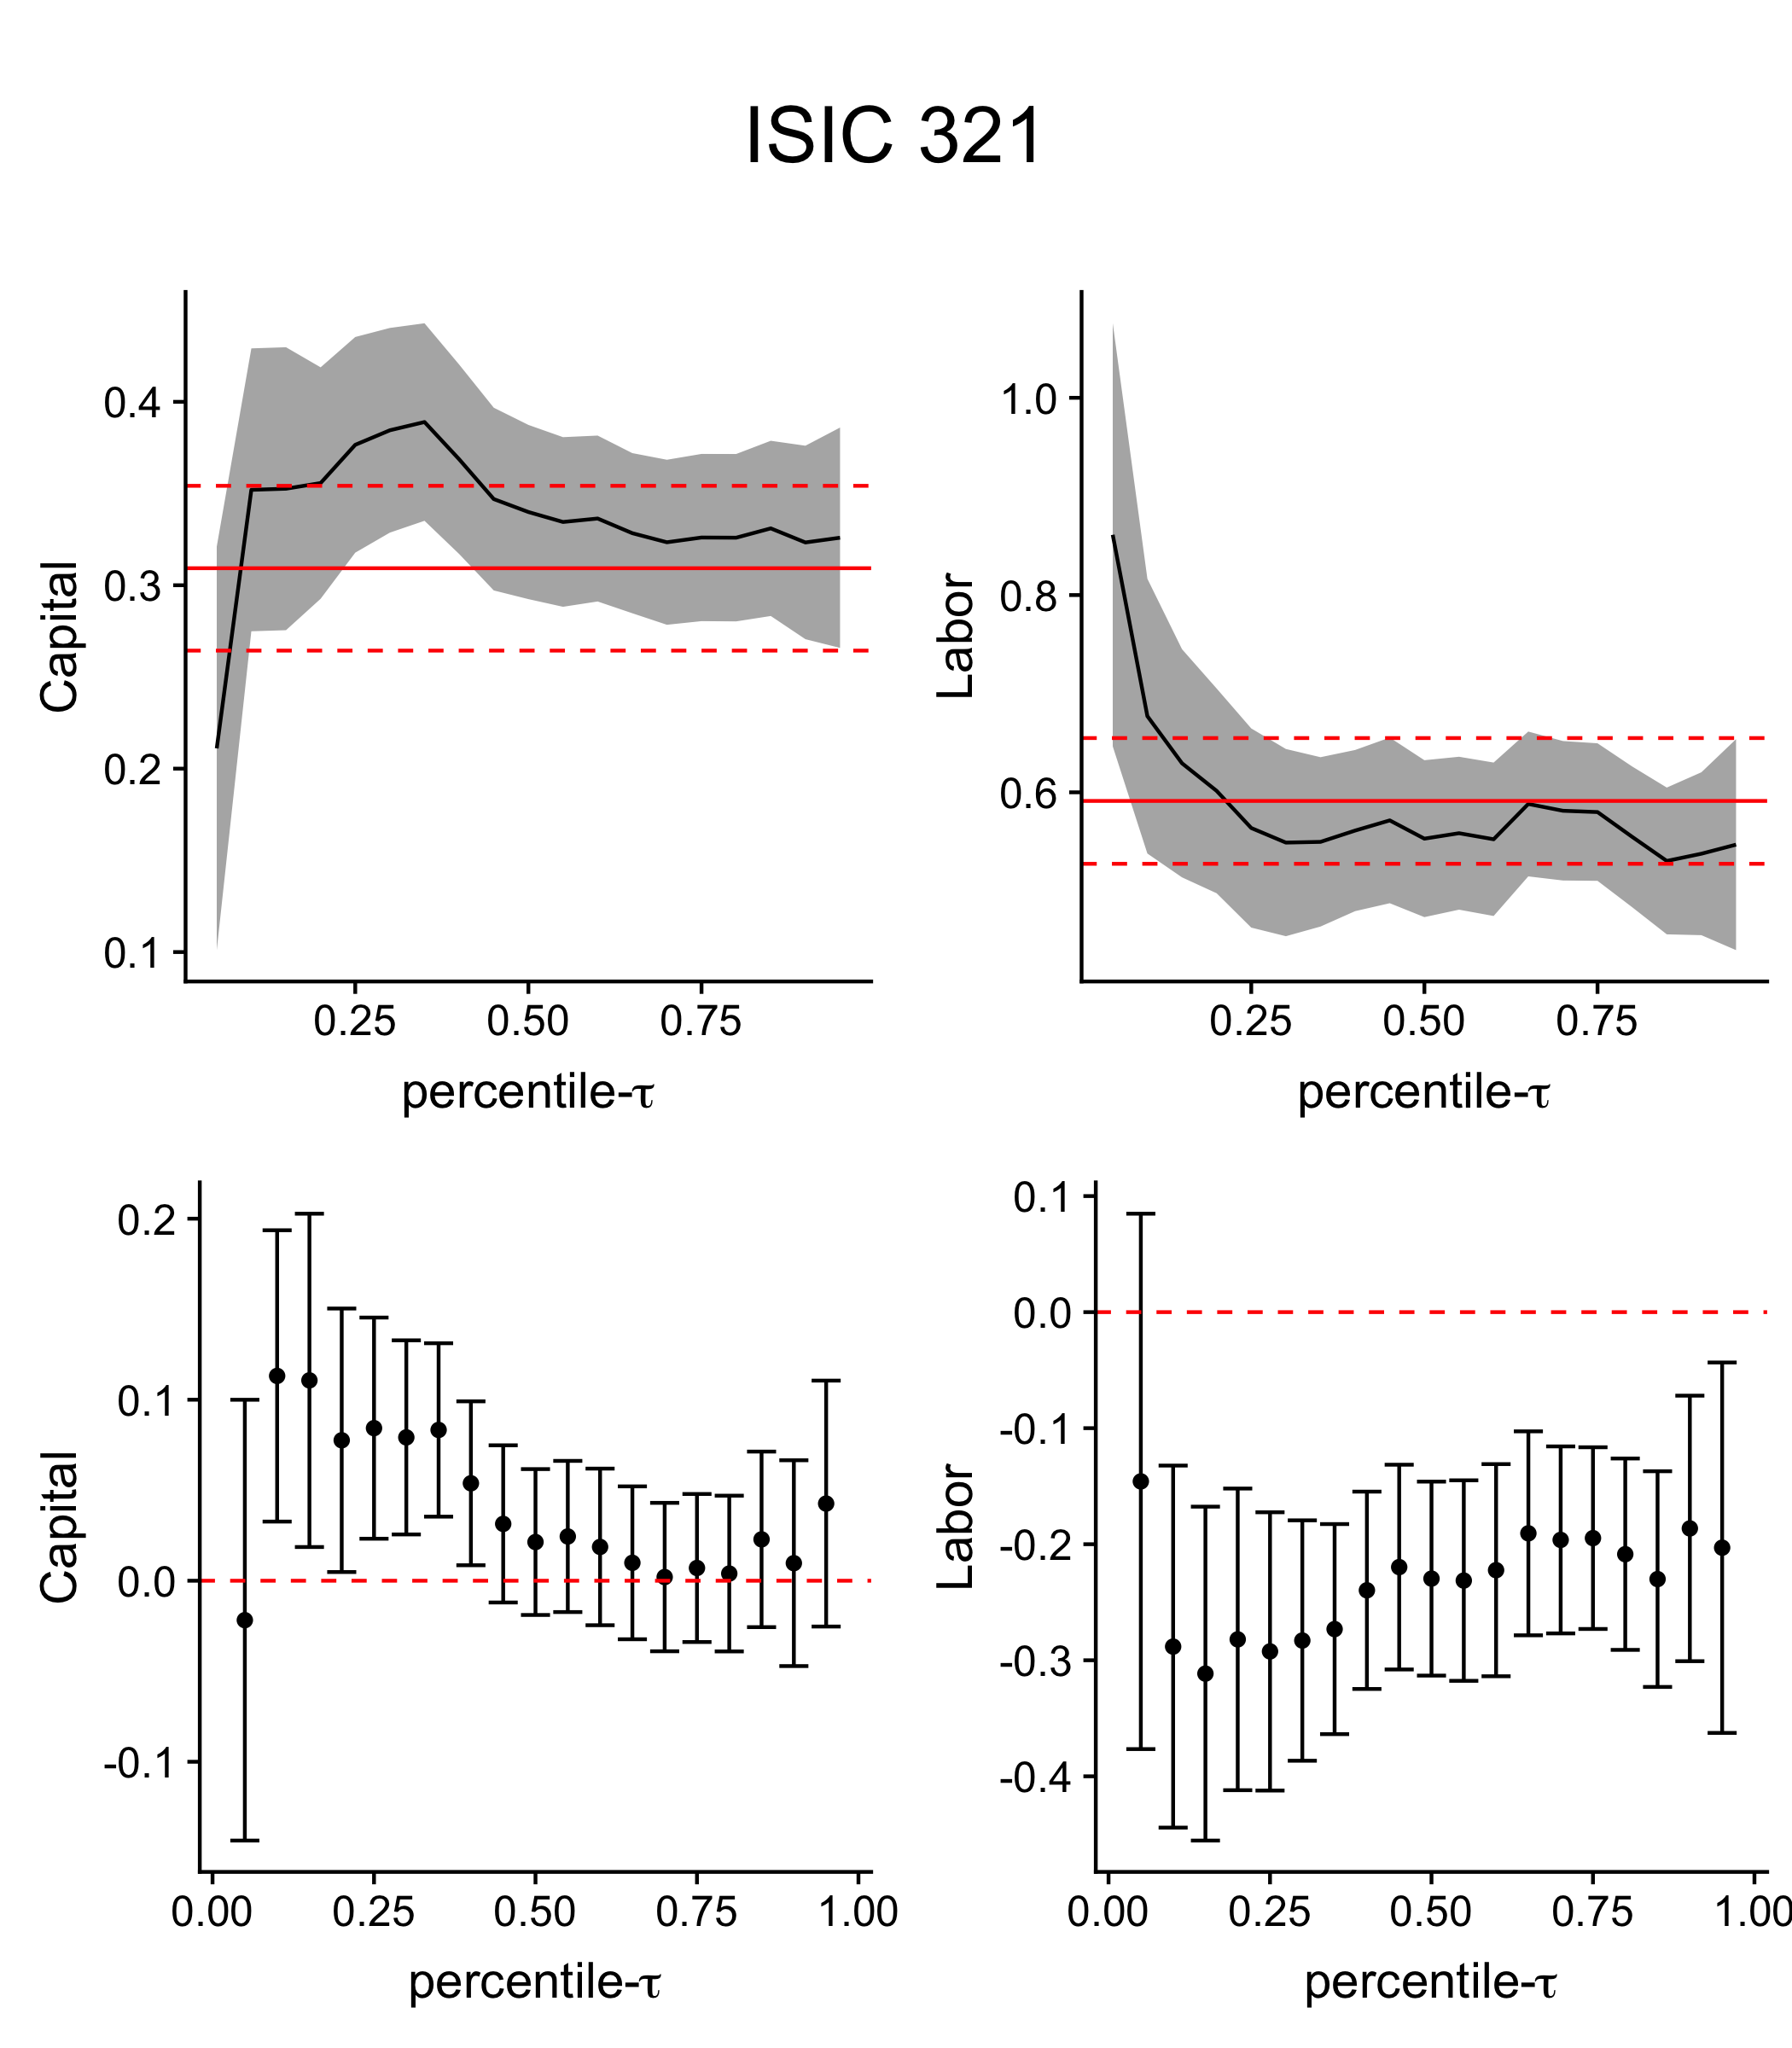
\includegraphics[width=12cm]{/Users/justindoty/Documents/Research/Dissertation/Production_QR_Proxy/Code/Empirical/Chile/Plots/Coef_Plot_ISIC_321.png}
\caption{Estimated values of production function coefficients and their 90\% confidence interval. The plots on the LHS are the QLP and LP estimates. The plots on the RHS are quantile regression and OLS estimates.}
\end{figure}

\begin{figure}[H]
\centering
\includegraphics[width=12cm]{/Users/justindoty/Documents/Research/Dissertation/Production_QR_Proxy/Code/Empirical/Chile/Plots/Coef_Plot_ISIC_381.png}
\caption{Estimated values of production function coefficients and their 90\% confidence interval. The plots on the LHS are the QLP and LP estimates. The plots on the RHS are quantile regression and OLS estimates.}
\end{figure}

\begin{figure}[H]
\centering
\includegraphics[width=12cm]{/Users/justindoty/Documents/Research/Dissertation/Production_QR_Proxy/Code/Empirical/Chile/Plots/Coef_Plot_ISIC_All.png}
\caption{Estimated values of production function coefficients and their 90\% confidence interval. The plots on the LHS are the QLP and LP estimates. The plots on the RHS are quantile regression and OLS estimates.}
\end{figure}

\begin{figure}[H]
\centering
\includegraphics[width=12cm]{/Users/justindoty/Documents/Research/Dissertation/Production_QR_Proxy/Code/Empirical/Chile/Plots/TFP_Plot.png}
\caption{Estimated average TFP over time for Chile. Base productivity in 1979 is set to 100.}
\end{figure}

\begin{figure}[H]
\centering
\includegraphics[width=12cm]{/Users/justindoty/Documents/Research/Dissertation/Production_QR_Proxy/Code/Empirical/Chile/Plots/Q3Q1_Grid_plot.png}
\caption{Estimated 75/25 productivity dipersion ratio and their 90\% confidence interval by industry.}
\end{figure}

\begin{figure}[H]
\centering
\includegraphics[width=12cm]{/Users/justindoty/Documents/Research/Dissertation/Production_QR_Proxy/Code/Empirical/Chile/Plots/Q9Q1_Grid_plot.png}
\caption{Estimated 90/10 productivity dipersion ratio and their 90\% confidence interval by industry.}
\end{figure}

\begin{figure}[H]
\centering
\includegraphics[width=12cm]{/Users/justindoty/Documents/Research/Dissertation/Production_QR_Proxy/Code/Empirical/Chile/Plots/Q95Q05_Grid_plot.png}
\caption{Estimated 95/5 productivity dipersion ratio and their 90\% confidence interval by industry.}
\end{figure}

\begin{figure}[H]
\centering
\includegraphics[width=12cm]{/Users/justindoty/Documents/Research/Dissertation/Production_QR_Proxy/Code/Empirical/Chile/Plots/Time_Plot.png}
\caption{Estimated values of production function coefficients over time estimated at 2 year intervals}
\end{figure}


%------------------------------------------------------------------------------------------------

\subsection{Colombia Manufacturing}

% latex table generated in R 3.4.1 by xtable 1.8-2 package
% Wed Jan  6 11:46:20 2021
\begin{table}[H]
\centering
\caption{Summary Statistics (in logs) for Colombia Manufacturing Data} 
\begin{tabular}{ccccccc}
  \hline\hline Industry (ISIC code) &   & 1st Qu. & Median & 3rd Qu. & Mean & sd \\ 
  \hline
311 (Total=13215) & Output & 9.03 & 10.21 & 11.59 & 10.42 & 1.8 \\ 
   & Capital & 8.69 & 9.37 & 10.22 & 9.49 & 1.18 \\ 
   & Labor & 8.52 & 9.3 & 10.33 & 9.54 & 1.43 \\ 
   & Materials & 8.7 & 9.62 & 10.88 & 9.92 & 1.67 \\ 
  322 (Total=12182) & Output & 6.02 & 7.07 & 8.35 & 7.24 & 1.78 \\ 
   & Capital & 5.47 & 6.14 & 6.93 & 6.23 & 1.21 \\ 
   & Labor & 5.89 & 6.75 & 7.81 & 6.93 & 1.55 \\ 
   & Materials & 5.9 & 6.89 & 8.16 & 7.12 & 1.77 \\ 
  381 (Total=7411) & Output & 2.56 & 3.09 & 3.97 & 3.36 & 1.1 \\ 
   & Capital & 2.77 & 3.3 & 3.95 & 3.42 & 0.92 \\ 
   & Labor & 2.64 & 3.18 & 3.91 & 3.37 & 0.98 \\ 
   & Materials & 2.71 & 3.3 & 4.11 & 3.5 & 1.09 \\ 
  All (Total=87783) & Output & 8.39 & 9.73 & 11.26 & 9.87 & 2 \\ 
   & Capital & 7.62 & 8.53 & 9.46 & 8.48 & 1.51 \\ 
   & Labor & 7.77 & 8.65 & 9.72 & 8.8 & 1.58 \\ 
   & Materials & 7.89 & 8.93 & 10.26 & 9.15 & 1.88 \\ 
   \hline
\end{tabular}
\end{table}

% latex table generated in R 3.4.1 by xtable 1.8-2 package
% Wed Mar  3 23:23:10 2021
\begin{table}[ht]
\centering
\caption{Coefficient Estimates and Standard Errors for Colombian Manufacturing Firms} 
\begin{tabular}{cccccccccc}
  \hline\hline & & \multicolumn{2}{c}{Capital}  & \multicolumn{2}{c}{Labor} & \multicolumn{2}{c}{Returns to Scale} & \multicolumn{2}{c}{Capital Intensity}\\ \cmidrule(lr){3-4} \cmidrule(lr){5-6} \cmidrule(lr){7-8} \cmidrule(lr){9-10}ISIC & $\tau$ & Coef. & s.e & Coef. & s.e & Coef. & s.e & Coef. & s.e \\ 
  \hline
311 & 0.10 & 0.165 & 0.0283 & 0.641 & 0.0361 & 0.805 & 0.0361 & 0.257 & 0.0530 \\ 
   & 0.25 & 0.234 & 0.0267 & 0.619 & 0.0202 & 0.853 & 0.0300 & 0.378 & 0.0476 \\ 
   & 0.50 & 0.323 & 0.0268 & 0.532 & 0.0185 & 0.855 & 0.0293 & 0.608 & 0.0582 \\ 
   & 0.90 & 0.510 & 0.0286 & 0.350 & 0.0302 & 0.860 & 0.0326 & 1.457 & 0.1759 \\ 
  322 & 0.10 & 0.148 & 0.0246 & 0.691 & 0.0298 & 0.839 & 0.0310 & 0.214 & 0.0394 \\ 
   & 0.25 & 0.213 & 0.0253 & 0.668 & 0.0272 & 0.881 & 0.0290 & 0.319 & 0.0434 \\ 
   & 0.50 & 0.311 & 0.0259 & 0.586 & 0.0277 & 0.897 & 0.0287 & 0.530 & 0.0562 \\ 
   & 0.90 & 0.506 & 0.0332 & 0.421 & 0.0442 & 0.927 & 0.0320 & 1.203 & 0.1780 \\ 
  381 & 0.10 & 0.150 & 0.0402 & 0.952 & 0.0588 & 1.102 & 0.0529 & 0.158 & 0.0471 \\ 
   & 0.25 & 0.259 & 0.0360 & 0.872 & 0.0356 & 1.131 & 0.0450 & 0.297 & 0.0446 \\ 
   & 0.50 & 0.366 & 0.0362 & 0.762 & 0.0327 & 1.127 & 0.0434 & 0.480 & 0.0538 \\ 
   & 0.90 & 0.509 & 0.0398 & 0.661 & 0.0417 & 1.171 & 0.0436 & 0.770 & 0.0861 \\ 
  All & 0.10 & 0.091 & 0.0118 & 0.748 & 0.0146 & 0.839 & 0.0136 & 0.122 & 0.0173 \\ 
   & 0.25 & 0.178 & 0.0110 & 0.715 & 0.0104 & 0.893 & 0.0121 & 0.248 & 0.0172 \\ 
   & 0.50 & 0.263 & 0.0109 & 0.654 & 0.0090 & 0.916 & 0.0116 & 0.402 & 0.0194 \\ 
   & 0.90 & 0.410 & 0.0120 & 0.573 & 0.0125 & 0.983 & 0.0122 & 0.715 & 0.0321 \\ 
   \hline
\end{tabular}
\end{table}


\begin{figure}[H]
\centering
\includegraphics[width=12cm]{/Users/justindoty/Documents/Research/Dissertation/Production_QR_Proxy/Code/Empirical/Colombia/Plots/Coef_Plot_ISIC_311.png}
\caption{Estimated values of production function coefficients and their 90\% confidence interval. The plots on the LHS are the QLP and LP estimates. The plots on the RHS are quantile regression and OLS estimates.}
\end{figure}

\begin{figure}[H]
\centering
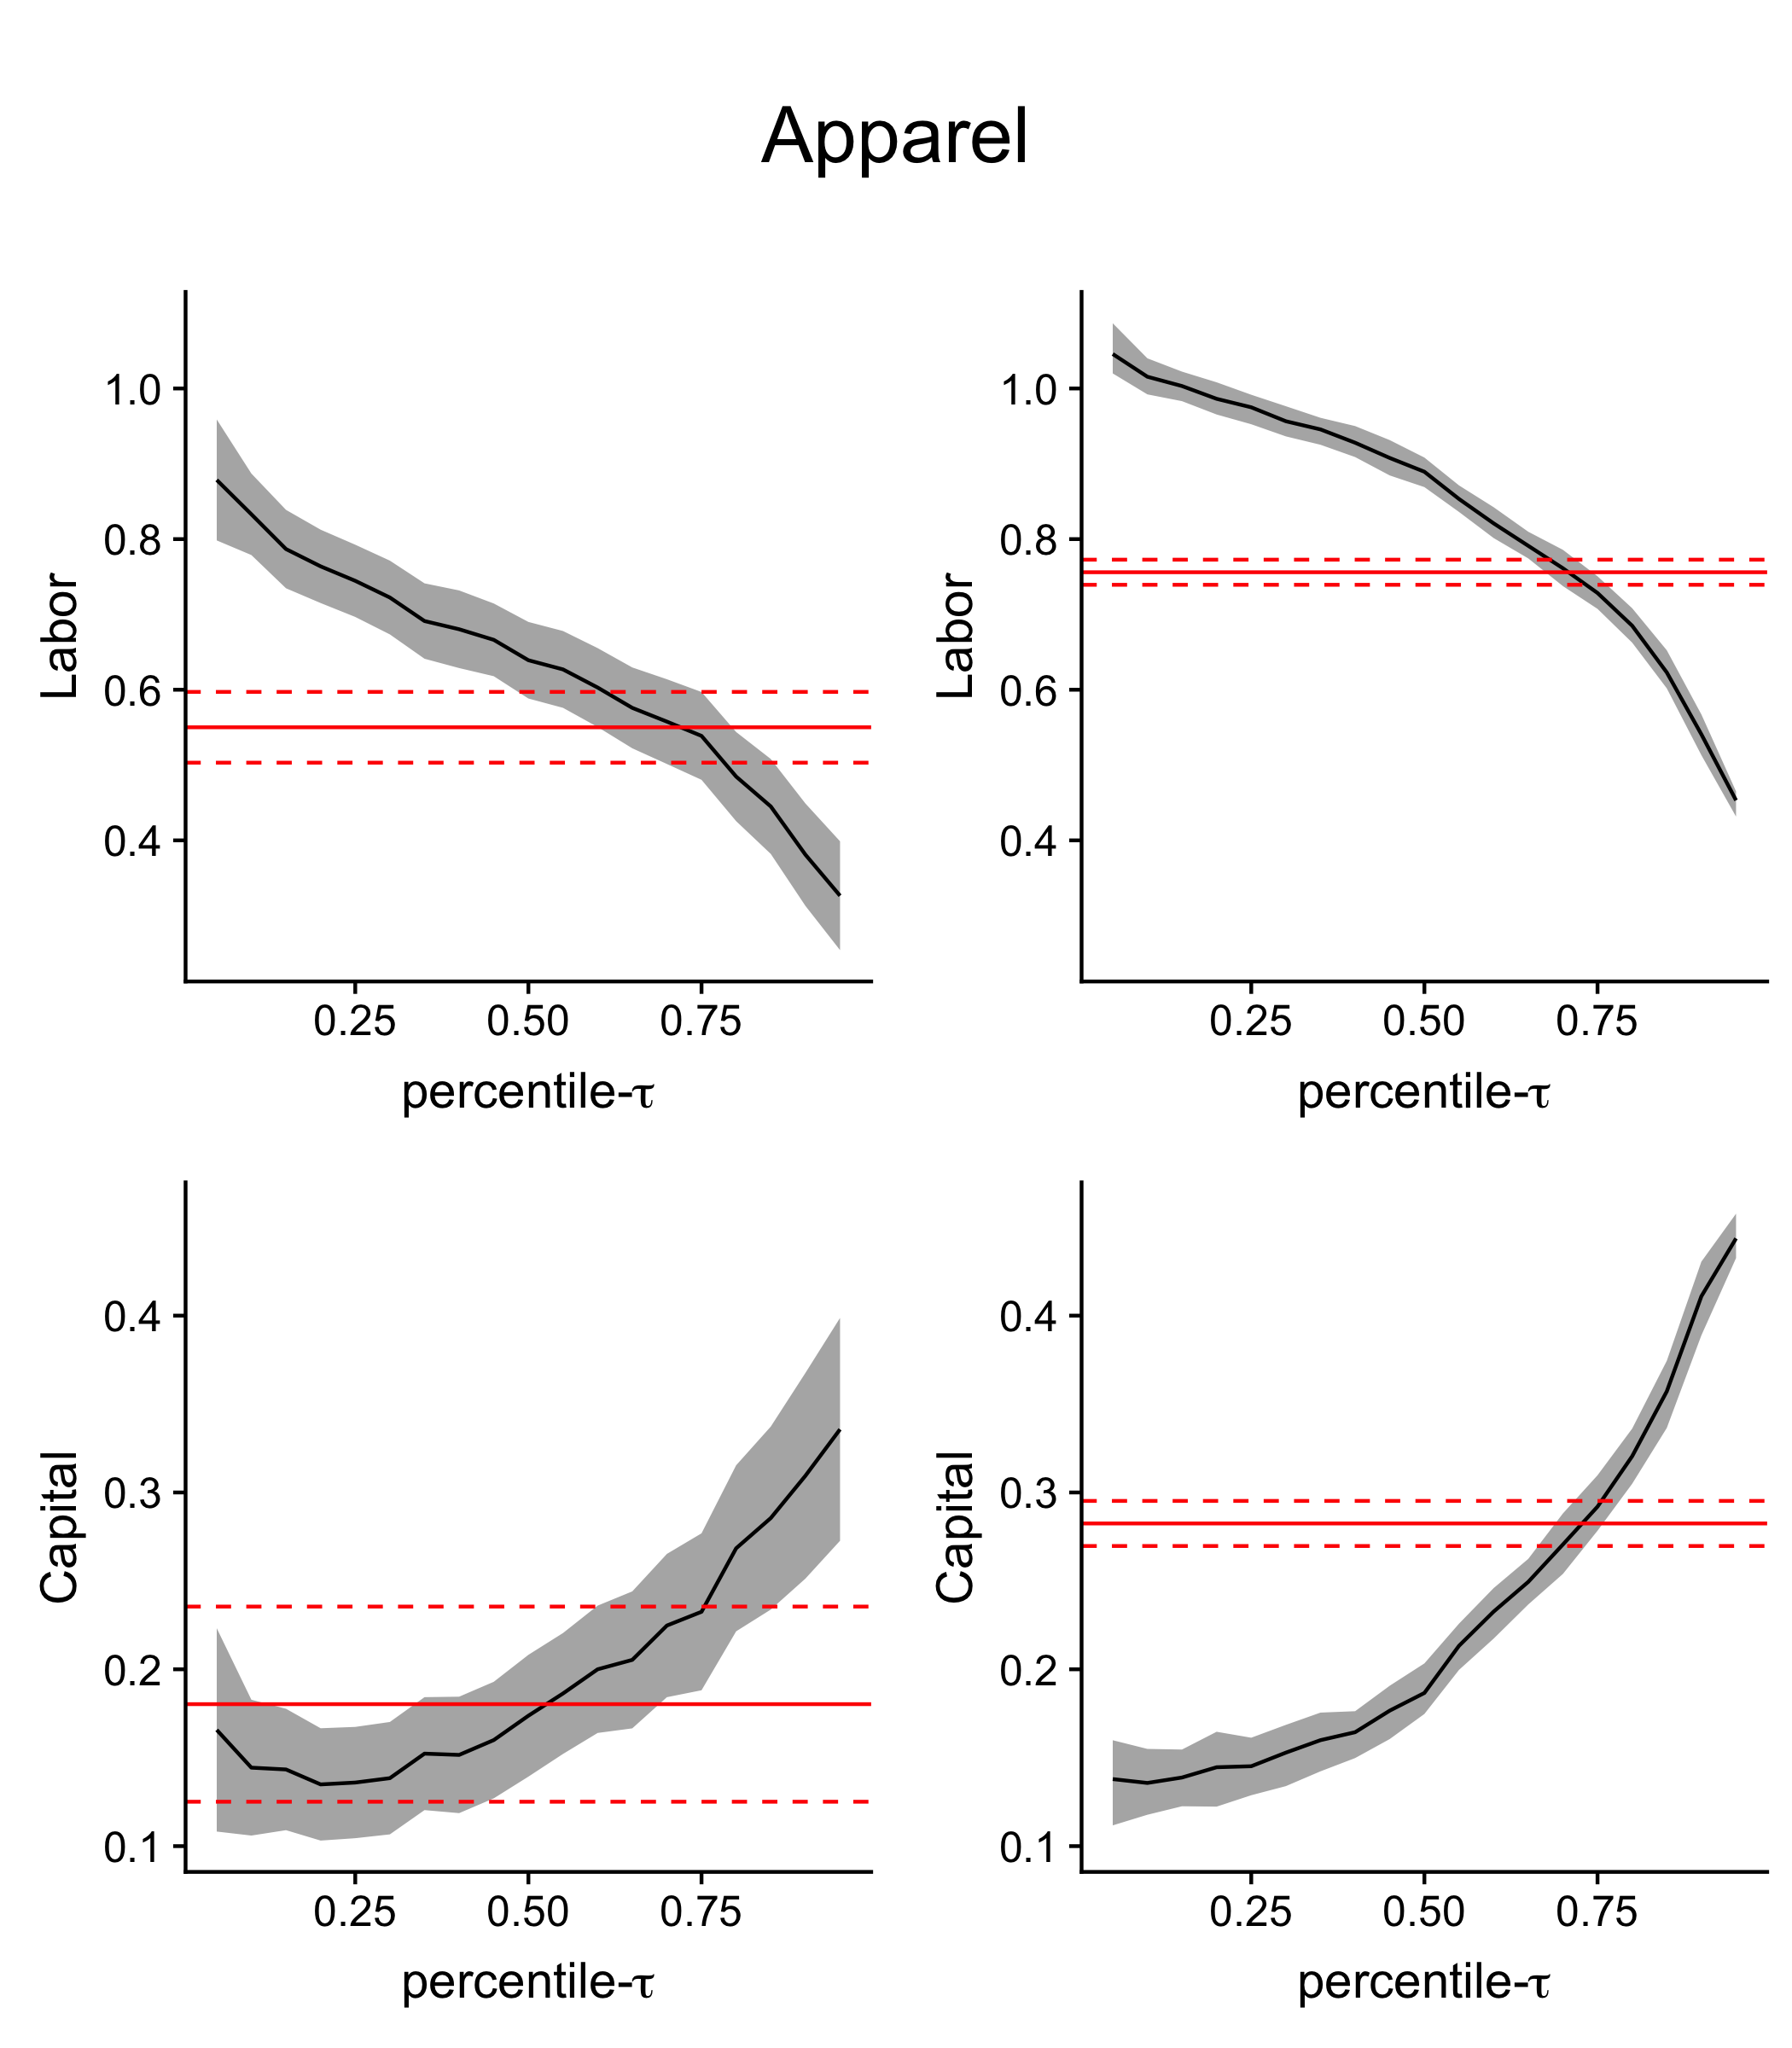
\includegraphics[width=12cm]{/Users/justindoty/Documents/Research/Dissertation/Production_QR_Proxy/Code/Empirical/Colombia/Plots/Coef_Plot_ISIC_322.png}
\caption{Estimated values of production function coefficients and their 90\% confidence interval. The plots on the LHS are the QLP and LP estimates. The plots on the RHS are quantile regression and OLS estimates.}
\end{figure}

\begin{figure}[H]
\centering
\includegraphics[width=12cm]{/Users/justindoty/Documents/Research/Dissertation/Production_QR_Proxy/Code/Empirical/Colombia/Plots/Coef_Plot_ISIC_381.png}
\caption{Estimated values of production function coefficients and their 90\% confidence interval. The plots on the LHS are the QLP and LP estimates. The plots on the RHS are quantile regression and OLS estimates.}
\end{figure}

\begin{figure}[H]
\centering
\includegraphics[width=12cm]{/Users/justindoty/Documents/Research/Dissertation/Production_QR_Proxy/Code/Empirical/Colombia/Plots/Coef_Plot_ISIC_All.png}
\caption{Estimated values of production function coefficients and their 90\% confidence interval. The plots on the LHS are the QLP and LP estimates. The plots on the RHS are quantile regression and OLS estimates.}
\end{figure}

\begin{figure}[H]
\centering
\includegraphics[width=12cm]{/Users/justindoty/Documents/Research/Dissertation/Production_QR_Proxy/Code/Empirical/Colombia/Plots/TFP_Plot.png}
\caption{Estimated average TFP over time for Colombia. Base productivity in 1978 is set to 100.}
\end{figure}

\begin{figure}[H]
\centering
\includegraphics[width=12cm]{/Users/justindoty/Documents/Research/Dissertation/Production_QR_Proxy/Code/Empirical/Colombia/Plots/Q3Q1_Grid_plot.png}
\caption{Estimated 75/25 productivity dipersion ratio and their 90\% confidence interval by industry.}
\end{figure}

\begin{figure}[H]
\centering
\includegraphics[width=12cm]{/Users/justindoty/Documents/Research/Dissertation/Production_QR_Proxy/Code/Empirical/Colombia/Plots/Q9Q1_Grid_plot.png}
\caption{Estimated 90/10 productivity dipersion ratio and their 90\% confidence interval by industry.}
\end{figure}

\begin{figure}[H]
\centering
\includegraphics[width=12cm]{/Users/justindoty/Documents/Research/Dissertation/Production_QR_Proxy/Code/Empirical/Colombia/Plots/Q95Q05_Grid_plot.png}
\caption{Estimated 95/5 productivity dipersion ratio and their 90\% confidence interval by industry.}
\end{figure}

\begin{figure}[H]
\centering
\includegraphics[width=12cm]{/Users/justindoty/Documents/Research/Dissertation/Production_QR_Proxy/Code/Empirical/Colombia/Plots/Time_Plot.png}
\caption{Estimated values of production function coefficients over time estimated at 2 year intervals}
\end{figure}

\section{Conclusions} \label{conclusion}

We proposed a method that extends the intermediate input proxy variable approach to estimating quantiles of the conditional quantiles of firm production. The method is computationally attractive as it resembles the two-stage estimator introduced in the control function literature with conditional quantile restrictions at each stage. As a result, practitioners are able to easily apply the proposed estimator to production function models where the data reveal significant heterogeneous output elasticities along the conditional distribution of firm's output. We showed that this estimator works well in finite samples by replicating the experiment of ACF (2015) and showing that it captures heterogeneity in firm-size under different data generating processes.  

Econometric issues with this estimator are currently being explored. A method to consistently estimate the long-run variance of the sample moment conditions to achieve the semi-parametric efficiency bound under general conditions is desired and extending the asymptotic results of \cite*{qgmm} might not be straightforward. We also seek to estimate and interpret the resulting estimates of total factor productivity. Once these are addressed, an application using data such as the Chilean firm-level data may reveal heterogeneity in production technology along the distribution of firm output. 
We leave them as future research agenda.


\pagebreak
\newpage



%\section*{Appendix}
%\appendix
%\begin{Large}
%\noindent \textbf{A. Proof of the Theorems}
%\end{Large}

%\counterwithin{theorem}{section}
%\section{Proofs}





\bibliographystyle{ecca.bst}
\bibliography{references}




\end{document}